%add example for other file formats: embl, genbank and swissprot.
%
\documentclass[12pt,titlepage]{article}
\usepackage{a4wide,ifpdf,ifthen,comment,alltt,xspace,makeidx}
%\usepackage{times}

\usepackage{mathptmx}
\usepackage[scaled=.90]{helvet}
\usepackage{courier}

\usepackage{rotating}
\usepackage{prognames}
\usepackage{optionman}
\usepackage{verbatim}
\usepackage{listings}
%
\usepackage{hyperref,html,graphicx}
%begin{latexonly}
\ifpdf%
%end{latexonly}
\hypersetup{%
   colorlinks=true,
%   hyperindex,
%   urlcolor=blue,
   linkcolor=red,
%   pagecolor=blue,
%   citecolor=blue
 }%
%begin{latexonly}
%\else
%\hypersetup{%
%   colorlinks=true,
%   hyperindex,
%   urlcolor=black,
%   linkcolor=black,
%   pagecolor=black,
%   citecolor=black
% }%
\fi%
%end{latexonly}
%
%\def\Withregexp{}
\ifthenelse{\isundefined{\Withregexp}}{%
\newcommand{\Ignoreregexp}[1]{}
}{%
\newcommand{\Ignoreregexp}[1]{#1}
}

\newcommand{\ShowSort}[3]{\index{sort mode!#1}\texttt{\small #1}:&sort in #2scending order of #3}
\newcommand{\TTindex}[1]{\index{#1@\texttt{#1}}}
\newcommand{\Seqformkeyword}[1]{\texttt{\small #1}\index{#1@\texttt{#1}}}
\newcommand{\Seqfilename}[1]{\texttt{\small #1}\index{#1@\texttt{#1}}}
\newcommand{\Environmentvariable}[1]{\texttt{\small #1}\index{#1@\texttt{#1}}}
\newcommand{\Datatype}[1]{\texttt{\small #1}\index{#1@\texttt{#1}}}
\newcommand{\Selectionfunction}[1]{\texttt{\small #1}\index{#1@\texttt{#1}}}
\newcommand{\Function}[3]{#1:#2\to#3}
\newcommand{\Size}[1]{|#1|}
\newcommand{\Iff}{if and only if\xspace}
\newcommand{\Nats}{\textrm{I}\!\textrm{N}}
\newcommand{\LCP}[0]{\mathit{lcptab}}
\newcommand{\SUF}[0]{\mathit{suftab}}
\newcommand{\STI}[0]{\mathit{stitab}}
\newcommand{\STIone}[0]{\mathit{stitab1}}
\newcommand{\BCK}[0]{\mathit{bcktab}}
\newcommand{\PRJ}[0]{\mathit{prjtab}}
\newcommand{\TIS}[0]{\mathit{tistab}}
\newcommand{\OIS}[0]{\mathit{oistab}}
\newcommand{\BWT}[0]{\mathit{bwttab}}
\newcommand{\LLV}[0]{\mathit{llvtab}}
\newcommand{\SKP}[0]{\mathit{skptab}}
\newcommand{\ISO}[0]{\mathit{isotab}}
\newcommand{\SSP}[0]{\mathit{ssptab}}
\newcommand{\DES}[0]{\mathit{destab}}
\newcommand{\SDS}[0]{\mathit{sdstab}}
\newcommand{\CLD}[0]{\mathit{cldtab}}
\newcommand{\Xdrop}[0]{\mathit{Xdrop}}
\newcommand{\GenPerLen}[2]{#1_{\mathit{#2}}}
\newcommand{\PerSmall}[0]{\GenPerLen{p}{small}}
\newcommand{\PerLarge}[0]{\GenPerLen{p}{large}}
\newcommand{\LenSmall}[0]{\GenPerLen{\ell}{small}}
\newcommand{\LenLarge}[0]{\GenPerLen{\ell}{large}}
\newcommand{\WILDCARD}{\texttt{WILDCARD}\xspace}
\newcommand{\SEPARATOR}{\texttt{SEPARATOR}\xspace}
\newcommand{\VMSopt}[1]{\Showoption{#1}}
\newcommand{\EMBL}{\Showformattype{Embl}}
\newcommand{\SWISSPROT}{\Showformattype{Swissprot}}
\newcommand{\GENBANK}{\Showformattype{Genbank}}
\newcommand{\Prefixlength}[0]{\mathit{prefixlength}}
\newcommand{\Minclsize}[0]{\Showoptionarg{minclsize}}
\newcommand{\Maxclsize}[0]{\Showoptionarg{maxclsize}}
\newcommand{\PrintVol}[1]{#1}
\newcommand{\Indexfile}[1]{\mathit{indexname}.\texttt{#1}}
\newcommand{\EcoliKtwelve}[0]{\emph{Ecoli~K12}\index{Ecoli~K12}\xspace}
\newcommand{\EcoliH}[0]{\emph{Ecoli~O157:H7}\index{Ecoli~O157:H7}\xspace}
\newcommand{\Indexfilesixfr}[1]{\mathit{indexname.6fr}.\texttt{#1}}
\newcommand{\Maxerrorthreshold}[0]{25}
\newcommand{\MUM}[0]{\textit{MUM}\xspace}
\newcommand{\EXECUTE}[1]{}
\newcommand{\Recentdetails}[1]{See page \pageref{#1} for more details\xspace}
%
\newcommand{\Program}[2]{\index{#2@#1}}
%
\newcommand{\ArabicLabels}{
  \renewcommand{\labelenumi}{$(\arabic{enumi})$}
  \renewcommand{\theenumi}{(\arabic{enumi})}
}
%
\newcommand{\RomanLabels}{
  \renewcommand{\labelenumi}{$(\roman{enumi})$}
  \renewcommand{\theenumi}{(\roman{enumi})}
}

\newenvironment{Output}{%
\begin{scriptsize}
\begin{alltt}}{%
\end{alltt}
\end{scriptsize}%
\addvspace{-\medskipamount}
}

\newenvironment{LargeOutput}{%
 \begin{footnotesize}
 \begin{alltt}}{%
 \end{alltt}
 \end{footnotesize}%
 \addvspace{-\medskipamount}
}

\lstset{language=C,
        basicstyle=\ttfamily\footnotesize,
        stringstyle=\ttfamily,
        keywordstyle=\ttfamily,
        commentstyle=\ttfamily\itshape,
        showstringspaces=false}

\newcommand{\Explainerroropt}[2]{
If this option is used together with option \Showoption{l}, then
substring matches are sought such that the two instances of the match contain 
at most $k$ #1. Here the mandatory argument $k$ is a positive 
integer. If this option is used together with option \Showoption{complete},
then complete matches are sought, and the mandatory argument
$k$ specifies the number of #1\xspace allowed in the match. 
$k$ can have three different forms:
\begin{itemize}
\item
If $k$ is a positive integer, then this specifies the absolute 
number of #1\xspace allowed.
\item
If $k$ is of the form $i\mathtt{p}$, where $i$ is a positive integer, then 
up to $\frac{i}{100}\cdot m$ #1\xspace are allowed in a match. 
Here $m$ is the length of the
current query to be searched. Thus the character $\mathtt{p}$ specifies
the #2 rate as a percentage of the query length. 
This mode is called the \emph{percentage} search mode.
\item
If $k$ is of the form $i\mathtt{b}$, where $i$ is a positive integer, then 
in a first search phase, the minimum number, say $q$, of 
#1 is determined, which still delivers at least one match for the given query. 
Then all matches with exactly $q$ #1 are reported. The range of values for 
$q$ to try in the first phase can be controlled by the positive integer.
That is, $q$ must be smaller than or equal to
$\frac{i}{100}\cdot m$.
This mode is called the \emph{best} search mode.
\end{itemize}
}

%begin{latexonly}
%
\ifthenelse{\isundefined{\BuildMkvtreeman}}{%
%For a complete manual use the following two lines
\includecomment{AboutVmatch}
\excludecomment{AboutMkvtree}
\newcommand{\AboutVmatchcmd}[1]{#1}
\newcommand{\AboutMkvtreecmd}[1]{}
\newcommand{\AboutMkdnasixcmd}[1]{}
}{%
%For a manual excluding \VM use the following two lines
\excludecomment{AboutVmatch}
\includecomment{AboutMkvtree}
\newcommand{\AboutVmatchcmd}[1]{}
\newcommand{\AboutMkvtreecmd}[1]{#1}
}
%end{latexonly}
%
\author{\begin{tabular}{c}
         \emph{Stefan Kurtz}\\
         Center for Bioinformatics,\\
         University of Hamburg,\\
         Bundesstrasse 43, 20146 Hamburg, Germany,\\
         E-mail: kurtz@zbh.uni-hamburg.de
        \end{tabular}}
\title{%
\AboutVmatchcmd{\textbf{The \emph{Vmatch} large scale sequence analysis software}\\[1cm] }
\AboutMkvtreecmd{\textbf{Construction of Virtual Suffix Trees}\\[1cm] }
\textbf{A Manual}
}
\makeindex
\begin{document}
\pagestyle{headings}
\maketitle
\newpage
\pagenumbering{Roman}
\tableofcontents

\newpage
\pagestyle{empty}

\pagestyle{headings}
\pagenumbering{arabic}
\setcounter{page}{1}

\section{Introduction}

This document describes \emph{Vmatch}, a versatile 
software tool for efficiently
solving large scale se\-quence matching tasks. 
\emph{Vmatch} subsumes the software tool
\emph{REPuter} \cite{KUR:CHO:OHL:SCHLE:STO:GIE:2001}
but is much more general, with a very flexible user interface,
and improved space and time requirement. Here are the most important
features of \emph{Vmatch}.

%%%BEGIN{introduction}

\begin{AboutVmatch}

\subsection*{Persistent index}
Usually, in a large scale matching problem, extensive portions of the sequences
under consideration are static, i.e.\ they do not change much over time. 
Therefore it makes sense to preprocess this static data
to extract information from it and to store this in a structured manner,
allowing efficient searches.
%Such an approach is, for example, used in the 
%BLAST, \index{BLAST} which comes with a program 
%\emph{formatdb} to preprocess a set of database sequences.
\emph{Vmatch} does exactly this: it preprocesses a set of sequences
into an index structure. This is stored as a collection of several files
constituting the persistent index. The index efficiently represents all 
substrings of the preprocessed sequences and, unlike
many other sequence comparison tools, allows matching tasks to be solved
in time, \emph{independent} of the size of the index. Different matching
tasks require different parts of the index, but only the required parts
of the index are accessed during the matching process.

\subsection*{Alphabet independency}
Most software tools for sequence analysis are restricted to DNA
and/or protein sequences. In contrast, \emph{Vmatch} can process sequences
over any user defined alphabet not larger than 250 symbols.
\emph{Vmatch} fully implements the concept of \emph{symbol mappings},
denoting alphabet transformations. These allow the user to specify that 
different characters in the input sequences should be considered identical 
in the matching process. This feature is used 
to group similar amino acids, for example.

\subsection*{Versatility}
\emph{Vmatch} allows a multitude of different matching tasks to be solved
using the persistent index. Every matching task is basically characterized by
(1) the \emph{kind of sequences} to be matched,
(2) the \emph{kind of matches} sought,
(3) additional \emph{constraints} on the matches, and
(4) the \emph{kind of postprocessing} to be done with the matches.

In the standard case, \emph{Vmatch} matches sequences over the same alphabet.
Additionally, DNA sequences can be matched against a protein sequence
index in all six reading frames. Finally, DNA sequences can be 
transformed in all six reading frames and compared against itself.

Where appropriate, \emph{Vmatch} can compute the
following kinds of matches, using state-of-the-art algorithms:

\begin{itemize}
\item
maximal and supermaximal repeats
using the algorithms of \cite{ABO:KUR:OHL:2004}.
\item
branching tandem repeats
using the algorithm of \cite{ABO:KUR:OHL:2002},
\item
maximal (unique) substring matches
using the algorithms of \cite{KUR:2002B}.
\item
complete matches
using the algorithms of \cite{MAN:MYE:1993} and \cite{MYE:1999}
\end{itemize}
To compute degenerate substring matches or degenerate repeats,
each kind of match (with the exception of tandem repeats and complete matches)
can be taken as an exact seed and extended by either
of two different strategies:
\begin{itemize}
\item
the \emph{maximum error} extension strategy, as described in 
\cite{KUR:CHO:OHL:SCHLE:STO:GIE:2001} for repeat detection,
\item
the \emph{greedy} extension strategy of \cite{ZHA:SCHWA:WAG:MIL:2000}.
\end{itemize}
Matches can be selected according to their length, their
E-value, their identity value, or match score.

In the standard case, a match is displayed as an alignment
including positional information.
Alternatively, a match can directly be postprocessed in
different ways:

\begin{itemize}
\item
\emph{inverse output}, i.e.\ reporting of substrings 
\emph{not} covered by a match.
\item
\emph{masking} of substrings covered by a match.
\item
\emph{clustering} of sequences according to the matches found.
\item
\emph{chaining} of matches, i.e.\ finding optimal subsets
of matches which do not cross, using the algorithms described in
\cite{ABO:OHL:2003}.
\item
\emph{clustering} of  matches according to pairwise sequence similarities
computed by the dynamic programming algorithm of \cite{UKK:1985A}.
\item
\emph{clustering} of matches according to the positions
where they occur, following the approach of 
\cite{VOL:HAA:SAL:2001}.
\end{itemize}

\subsection*{Efficient algorithms and data structures}
\emph{Vmatch} is based on enhanced suffix arrays
described  Abouelhoda, Kurtz \& Ohlebusch, 2004.
This data structure
has been shown to be as powerful as suffix trees, with the advantage of
a reduced space requirement and reduced processing time. Careful 
implementation of the algorithms and data structures incorporated in
\emph{Vmatch} have led to exceedingly fast and robust software,
allowing very large sequence sets to be processed quickly.
%For example, the two largest human
%chromosomes can be fully compared in less an hour on 2~GHz PC using
%2.4 gigabytes of main memory.
The 32-bit version of \emph{Vmatch} can process 
up to 400 million symbols, if enough memory is available.
For large server class machines (e.g.\ SUN-Sparc/Solaris,
Intel Xeon/Linux, Compaq-Alpha/Tru64) \emph{Vmatch} 
is available as a 64 bit version, enabling gigabytes of sequences
to be processed.

\subsection*{Flexible input format}
The most common formats for input sequences (Fasta, Genbank, EMBL, and
SWISSPROT) are accepted. The user does not have to specify the input
format. It is automatically recognized. All input files can contain
an arbitrary number of sequences. Gzipped compressed inputs are
accepted.

\subsection*{Customized output and match selection}
\emph{Vmatch}'s output can be parsed by other programs easily.
Furthermore, several options allow for its customization.
XML output is available and new output formats can easily be 
incorporated without changing \emph{Vmatch}'s
program code. Certain matches can easily be selected by
user defined criteria, without intermediate output and subsequent
parsing.

\subsection*{The parts of Vmatch}
Up until now we have referred to \emph{Vmatch} as a collection
of programs. In the following we use the same name, 
\texttt{vmatch} (in typewriter font), for the most important 
program in this collection. Besides \texttt{vmatch}, there are
the following programs available:
\begin{enumerate}
\item
\texttt{mkvtree} constructs the persistent index and stores it on files.
\item
\texttt{mkdna6idx} constructs an index for a DNA sequence 
after translating this in all six reading frames.
\item
\texttt{vseqinfo} delivers information about indexed database sequences.
\item
\texttt{vstree2tex} outputs a representation of the index
in \LaTeX-format. It can be used, for example, for educational
or debugging purposes.
\item
\texttt{vseqselect} selects indexed sequences satisfying specific
criteria.
\item
\texttt{vsubseqselect} selects substrings of a specified length range 
from an index. 
\item
\texttt{vmigrate.sh} converts an index from big endian to
little endian architectures, or vice versa.
\item
\texttt{vmatchselect} sort and selects matches 
delivered by \texttt{vmatch}.
\item
\texttt{chain2dim} computes optimal chains of matches from files
in \emph{Vmatch}-format.
\item
\texttt{matchcluster} computes clusters of matches from files
in \emph{Vmatch}-format.
\end{enumerate}

%%%END{introduction}

Figure \ref{VmatchDataflow} depicts the 
data flow in the different tools described
in this manual.

\begin{figure}
\caption{
The Dataflow in \emph{Vmatch}. The programs
are shown in ellipses. The inputs are the database
and the query sequences and the alphabet transformation,
represented by rectangles. At the center of all
computations the persistent index is shown. All other
rectangles represent the different kinds of output.}
\label{VmatchDataflow}
%begin{latexonly}
\ifpdf
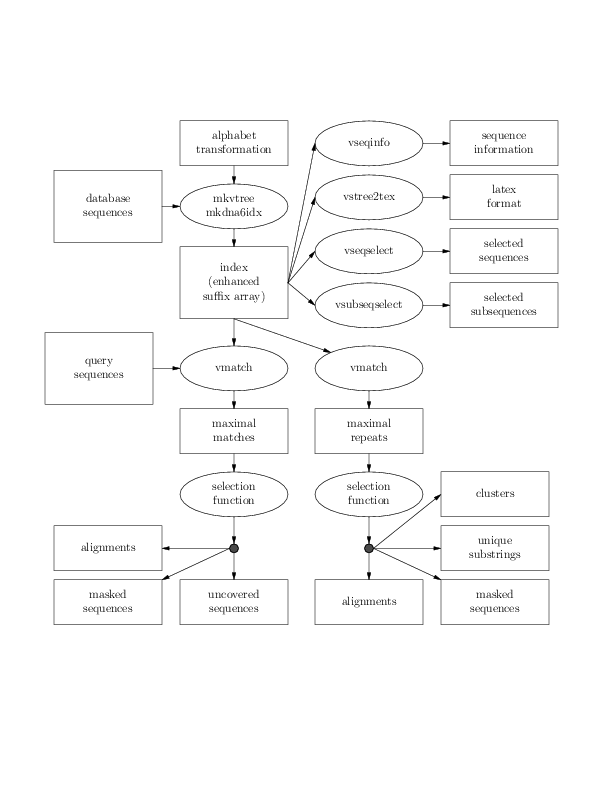
\includegraphics[width=\textwidth,height=\textheight]{Dataflow.png}
\else
\documentclass[12pt]{article}
\usepackage{a4wide}
\pagestyle{empty}
\begin{document}
\documentclass[12pt]{article}
\usepackage{a4wide}
\pagestyle{empty}
\begin{document}
\documentclass[12pt]{article}
\usepackage{a4wide}
\pagestyle{empty}
\begin{document}
\input{Dataflow.inc}

\centerline{\box\graph}
\end{document}


\centerline{\box\graph}
\end{document}


\centerline{\box\graph}
\end{document}

\centerline{\box\graph}
\fi
%end{latexonly}
\begin{htmlonly}
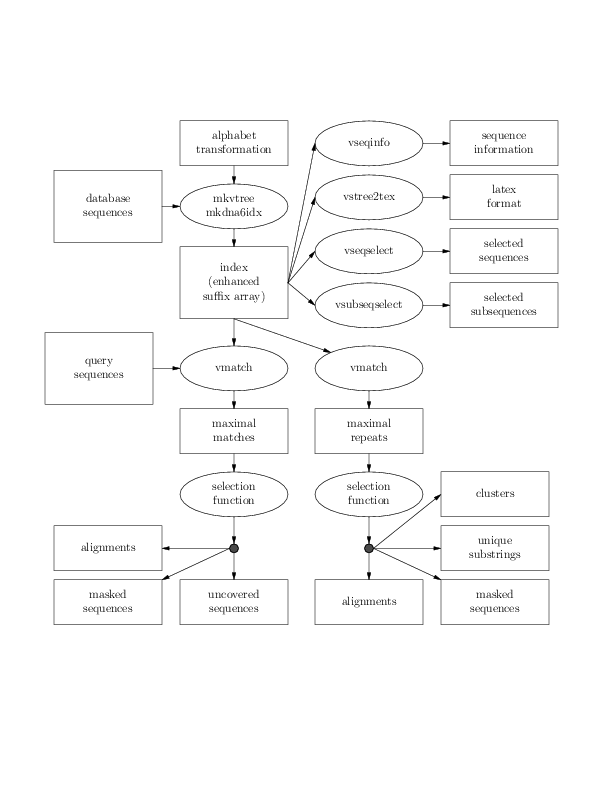
\includegraphics{Dataflow.png}
\end{htmlonly}
\end{figure}

\subsection*{Overview}
%There are two reasons for the name ``virtual suffix trees'': 
%First, as an index data structure we use a \index{suffix array}
%suffix array with additional information, but for
%searching we adopted algorithms, which were originally developed 
%for \index{suffix tree} suffix trees. Second, the index is stored on 
%different files, which are mapped into main memory. The virtual memory 
%management system takes care that only those portions of the index are 
%copied to main memory which are currently needed.

The rest of this
document is organized as follows: In Section \ref{MKV} we describe
\MKV, a program which constructs the index. For a DNA sequence
we can construct a six-frame index using the programming 
\MKDNASIX, described in section \ref{MKDNASIXSECTION}.
Section \ref{VSI} is devoted to
the program \VSI which delivers information about the indexed
database sequences.\index{database}
In Section 
\ref{VtoTex} we describe the program \VtoTex which outputs the tables
of a virtual suffix tree in \LaTeX-format.
Section \ref{VSS} is devoted to the program
\VSS which allows to select sequences from an index satisfying specific
criteria. Similarly, the program \VSSS described in Section \ref{VSSS}
selects substrings of a specified length range from an
index. Section \ref{VMI} describes the shell-script \VMI to convert
an index from big endian (e.g.\ \index{SUN} SUN/Sparc or \index{SGI} 
SGI/IRIX) to 
little endian (e.g.\ Linux \index{Linux} or \index{Compaq-Alpha} Compaq-Alpha)
architectures, or vice versa.
In Section \ref{VM} we explain
how to use the program \VM which allows to solve a variety of matching 
tasks on the index. Section \ref{VMS} is devoted to the program \VMS,
which allows to sort and select matches delivered by \VM.
Each of these sections is completed with several examples showing how
to apply the different programs to solve the different matching tasks.
In the course of this, the output format is explained.

In Appendix \ref{Basic} we define some basic notions. 
\Ignoreregexp{
Appendix \ref{Regexpdef} gives a precise definition of the
notion of regular expressions, as used in \VM.}
Appendix \ref{Symbolmap} explains the format of 
the symbol mapping.
Appendix \ref{Xdropextend} goes into detail about the 
\(X\)-drop extension strategy.
Substring Specifications are described in Appendix 
\ref{Substringspecifications}.
Appendix \ref{SelectionConcept} is devoted to the concept of
selection functions.
Finally Appendix \ref{TheTables} explains the tables 
the index consists of.
\end{AboutVmatch}

\section[\MKV]{\MKV: Making Virtual Suffix Trees}\label{MKV}\Program{\MKV}{mkvtree}
The program \MKV constructs an \index{index}
\emph{index} for a given set of sequences
These are given as a list of \emph{input files}. \index{file!input} 
The sequences are referred to as
\emph{database sequences}.
They can be over any given \index{alphabet} \emph{alphabet}.
The alphabet can be
the \index{alphabet!DNA} DNA alphabet, or the \index{alphabet!protein} 
protein alphabet, or any other alphabet consisting of printable characters.
An alphabet is specified by a file storing a 
\index{symbol mapping} \emph{symbol mapping}. The index consists of several 
files, the \index{file!index}
\emph{index files}. Each such file stores a different table.
The user specifies which tables (i.e.\ which part of the index)
is written to a file, using one of eight output options, or a single
option specifying that all tables are written to file. 
Appendix \ref{TheTables} gives a comprehensive description of
the different tables. We recommend the user to only use the
output options \Showoption{tis}, \Showoption{ois}, \Showoption{suf}, 
\Showoption{sti1}, \Showoption{bwt}, \Showoption{bck}, and \Showoption{lcp}.
Option \Showoption{skp} is only necessary for approximate pattern matching.

If an error occurs, the program exits with 
\index{error code} error code 1. Otherwise, the exit code is 0.
We support the following formats for the input files.
They are recognized according to the first non-white space symbol in 
the file. \index{input!format}

\label{Vmatchinputformat}
\begin{description}
\item[multiple \Fasta format]
\index{multiple fasta}
If the file begins with the symbol \Fastastart,
then this file is considered to be a file in multiple \Fasta format
(i.e.\ it contains one or more sequences). 
Each line starting with the symbol \Fastastart contains the 
\emph{description} of the sequence following it.
Each line not starting with the symbol \Fastastart contains the sequence.
Empty lines are allowed and ignored when reading the input.
\index{description!\Fasta}

\item[multiple \EMBL/\SWISSPROT format]
\index{EMBL@\EMBL}
\index{SWISSPROT@\SWISSPROT}
If the file begins with the string \Seqformkeyword{ID}, 
then this file is considered to be a file in multiple \EMBL format 
(i.e.\ containing one or more sequences, each in \EMBL-format). 
The information contained in
the \Seqformkeyword{ID} and \Seqformkeyword{DE}-lines is taken as the 
\emph{description} of the 
corresponding sequence. The \EMBL format is identical
to the \SWISSPROT format (w.r.t.\ the information we need to extract
from such entries). So one can also use files in multiple
\SWISSPROT format as input.
\index{description!\SWISSPROT}
\index{description!\EMBL}

\item[multiple \GENBANK format]
\index{GENBANK@\GENBANK}

If the file begins with the string \Seqformkeyword{LOCUS}, 
then this
file is considered to be a file in multiple \GENBANK format (i.e.\ containing
one or more entries in \GENBANK-format).
The information contained in the \Seqformkeyword{LOCUS} and the 
\Seqformkeyword{DEFINITION}-lines is taken as the 
\emph{description} of the corresponding sequence.
\index{description!\GENBANK}

\item[plain format]
If the file does not begin with the symbol 
\Fastastart or the strings \Seqformkeyword{ID} or 
\Seqformkeyword{LOCUS}, then the file is taken verbatim. That is, the
entire file is considered to be the input sequence (white spaces are 
\emph{not} ignored).
\end{description}

There is no special option necessary to tell the program the sequence format.
It automatically detects the appropriate format, according to the
rules given above. If none of the above rules apply, then the program
cannot recognize the input format and 
\index{error code} exits with error code 1. In such a case please
check you input files for if they are conform with the input formats
above. Another good solution is to use a more versatile
sequence format transformation programs (e.g.\ \Programname{readseq}) to 
first generate multiple \Fasta files and then feed this into \MKV.

Today many files containing sequence files are provided compressed
by the program \Programname{gzip}. To simplify the use of these files,
\MKV also accepts gzipped input files. These files must have the ending 
\texttt{.gz}.\index{input!gzipped} The gzipped formatted files are
gunzipped internally and then processed as any other file.
\label{Gzipinputformat}

\subsection{The Options of \MKV}

In this subsection, we describe the program \MKV by explaining its options. 
An option is always beginning with the dash symbol. 
We write an option in \texttt{typewriter} mode. Arguments to options
are written in typewriter mode if they are to be used verbatim.
We use \textit{italics} for an option argument if it is to be replaced by a 
some value. Table \ref{OverviewMKVopt} gives an overview of the
option available in \MKV. 

\begin{table}
\caption{Overview of the \MKV-Options}
\label{OverviewMKVopt}
\begin{footnotesize}
\begin{center}
\begin{tabular}{ll}\hline
\Showoption{db}& specify database files (mandatory)
\\
\Showoption{q}& specify query files
\\
\Showoption{smap}& specify file containing a symbol mapping
\\
\Showoption{dna}& input is DNA sequence
\\
\Showoption{protein}& input is Protein sequence
\\
\Showoption{indexname}& specify name for index to be generated
\\
\Showoption{pl}& specify prefix length for bucket sort
\\
\Showoption{rev}& use reverse input sequence
\\
\Showoption{tis}& output transformed input sequences (tistab) to file
\\
\Showoption{ois}& output original input sequences (oistab) to file
\\
\Showoption{suf}& output suffix array (suftab) to file
\\
\Showoption{sti1}& output reduced inverse suffix array (sti1tab) to file
\\
\Showoption{bwt}& output Burrows-Wheeler Transformation (bwttab) to file
\\
\Showoption{bck}& output bucket boundaries (bcktab) to file
\\
\Showoption{lcp}& output longest common prefix lengths (lcptab) to file
\\
\Showoption{skp}& output skip values (skptab) to file
\\
\Showoption{allout}& output all index tables to files
\\
\Showoption{v}& verbose mode
\\
\Showoption{help}& this option
\\
\hline
\end{tabular}

\end{center}
\end{footnotesize}
\end{table}

\begin{Showprogramwithoptionswithoutindex}{\MKV}{}

\Option{db}{\Showoptionarg{dbfiles}}{
Specify a non empty list of database files separated by white spaces.
Each database file contains sequences in one of the formats as
specified above. However, the format of all files has to 
be identical. The sequence must consist of characters
over the alphabet as specified by the options \Showoption{dna}, 
\Showoption{protein}, or \Showoption{smap}, see below.
White spaces are ignored. This option is mandatory.
\index{file!database}
}

\begin{comment}
\Option{q}{\Showoptionarg{queryfiles}}{
Specify a non empty list of query files separated by white space characters.
We suggest the splitting of the input files into database files and query 
files whenever the user has two sets of sequences between which several 
different matching tasks are to be performed. In this case, the user
can store these two sets in different files, and declare one set of files as
database files and the other as query files. In most cases, however, the user
will only specify database files for constructing the index. 
\index{file!query}
}
\end{comment}

\label{SMAPoption}
\Option{smap}{\Showoptionarg{mapfile}}{
Specify the file storing the symbol mapping.
\index{symbol mapping}
If the given \Showoptionarg{mapfile} cannot be found in the directory where
\MKV is run, then all directories specified by the environment variable
\Environmentvariable{MKVTREESMAPDIR}
are searched. If defined correctly, this contains a 
list of directory paths separated by colons (\texttt{`:'}). For example, 
if one uses the \Programname{csh} or the \Programname{tcsh}, 
the definition of the environment-variable could look like this:

\begin{LargeOutput}
\$ setenv MKVTREESMAPDIR \SY{34}\$HOME/vstree:/usr/vstree/TRANS\SY{34}
\end{LargeOutput}

For the \Programname{bash} or the \Programname{sh} the 
definition could look like

\begin{LargeOutput}
\$ MKVTREESMAPDIR=\SY{34}\$HOME/vstree:/usr/vstree/TRANS\SY{34}

\$ export MKVTREESMAPDIR
\end{LargeOutput}

Then, if \Showoptionarg{mapfile} is not available in the current directory, 
\MKV searches for \Showoptionarg{mapfile} in the two given directories. It
scans the directory-list from left to right. As soon as it has found the file
it stops. If the file cannot be found an error message is reported and
the program exits with \index{error code}
error code 1. See Appendix \ref{Symbolmap}
for a more detailed explanation of the format of the symbol mapping file.
}

\Option{dna}{}{
This option is equivalent to the option \Showoption{smap} 
\Showoptionarg{mapfile}
where \Showoptionarg{mapfile} stores exactly the following 5 lines:
}

\begin{LargeOutput}
aA
cC
gG
tTuU
nsywrkvbdhmNSYWRKVBDHM
\end{LargeOutput}

This specifies an alphabet of size 4 with additional \index{wildcard}
wildcard symbols appearing in the fifth line. 
See Appendix \ref{Symbolmap} for a more
detailed explanation of the format of the symbol mapping file. 

\medskip

\Option{protein}{}{
This option is equivalent to the option \Showoption{smap} 
\Showoptionarg{mapfile}
where \Showoptionarg{mapfile} stores exactly the following 21 lines:
}

\begin{LargeOutput}
L
V
I
F
K
R
E
D
A
G
S
T
N
Q
Y
W
P
H
M
C
XUBZJO*-
\end{LargeOutput}

This specifies an alphabet of size 20 with additional \index{wildcard}
wildcard symbols on
the last line.  See Appendix \ref{Symbolmap} for a more detailed
explanation of the format of the symbol mapping file.

\medskip

\Option{indexname}{\Showoptionarg{filepath}}{
Specify \Showoptionarg{filepath} to be the name of the index, later referred
to by \emph{indexname}. This option is mandatory, if 
more than one database 
%or query 
file is given and if additionally at least one file comprising the 
index is stored (i.e.\ if any of the output options is used). If no 
file from the index is stored, then this option is not allowed. 
If there is only one database file, and this option is not given, then 
\emph{indexname} is the basename of the given \Showoptionarg{filepath},
i.e.\ the filename stripped by the directory path where it is stored. 
The \Showoptionarg{filepath} can be a complete path.
}

\label{PLoption}
\Option{pl}{$\Showoptionalarg{prefixlength}$}{
Start the sorting of the suffixes with a initial step that sort all
suffixes according to their prefixes of length 
\Showoptionarg{prefixlength}. The argument \Showoptionarg{prefixlength} is
optional. Hence it is denoted in square brackets.
If the argument is omitted, then the value
for \Showoptionarg{prefixlength} is automatically determined. More precisely,
it is \(\left\lfloor\log_{k}\frac{n}{8}\right\rfloor\), 
where \(n\) is the total length of the database sequences and 
\(k\) is the alphabet size ($k=4$ for DNA, $k=20$ for proteins, and $k=$
one less than the number of lines in the corresponding symbol mapping 
file). Table \ref{Automaticprefixlength} shows the choices 
for the \Showoptionarg{prefixlength} for DNA and protein sequences,
given different ranges of values for \(n\).
\begin{table}
\caption{The value of $\Prefixlength$ automatically determined for
different ranges for DNA and proteins and different input sizes.}
\label{Automaticprefixlength}
\begin{center}
\begin{small}
\begin{tabular}{cc}
\begin{tabular}[t]{|l|r|}\hline
\multicolumn{2}{|c|}{DNA}\\\hline\hline
range of $n$ & $\Prefixlength$\\\hline
$513-2{,}048$ & 4 \\\hline
$2{,}049-8{,}192$ & 5 \\\hline
$8{,}193-32{,}768$ & 6 \\\hline
$32{,}769-131{,}072$ & 7 \\\hline
$131{,}073-524{,}288$ & 8 \\\hline
$524{,}289-2{,}097{,}152$ & 9 \\\hline
$2{,}097{,}153-8{,}388{,}608$ & 10 \\\hline
$8{,}388{,}609-33{,}554{,}432$ & 11 \\\hline
$33{,}554{,}433-134{,}217{,}728$ & 12 \\\hline
$134{,}217{,}729-536{,}870{,}912$ & 13 \\\hline
\end{tabular}&
\begin{tabular}[t]{|l|r|}\hline
\multicolumn{2}{|c|}{protein}\\\hline\hline
range of $n$ & $\Prefixlength$\\\hline
$161-3{,}200$ & 2 \\\hline
$3{,}201-64{,}000$ & 3 \\\hline
$64{,}001-1{,}280{,}000$ & 4 \\\hline
$1{,}280{,}001-25{,}600{,}000$ & 5 \\\hline
\end{tabular}
\end{tabular}
\end{small}
\end{center}
\end{table}
The maximum value for \(\Prefixlength\) is
\(\left\lfloor\log_{k}\frac{4n}{8}\right\rfloor\).
If you want to choose the prefix length manually, then
we recommend \(\Prefixlength\in[4,13]\) for DNA sequences, and
\(\Prefixlength\in[2,5]\) for protein sequences, depending on the
total length of the input sequences, see Table \ref{Automaticprefixlength}.
If this option is not specified, then the value for \(\Prefixlength\) is
\(0\), in which case no initial bucket sort is 
performed.
Note that in case you want to match a query against the index, the 
least length for the search must be at least $\Prefixlength$. 

%The maximum value for
%$\Prefixlength$ is $\min(15,\lfloor\log_{k}(2^{\omega-4}-1)\rfloor)$,
%where \(\omega\) is the integer size the program was compiled with 
%(32 or 64 bit) and \(k\) is the alphabet size of the sequence to process. 
%So, for a DNA sequence with an alphabet of size 4 
%and a program using 32-bit integers, the maximum prefix length is 
%$\min(15,\lfloor\log_{4}(2^{32-4}-1)\rfloor)$
}

\Option{tis}{}{
Store the table \(\TIS\) in file \(\Indexfile{tis}\).
}

\Option{ois}{}{
Store the table \(\OIS\) in file \(\Indexfile{ois}\).
}

\Option{suf}{}{
Store the table \(\SUF\) in file \(\Indexfile{suf}\).
}

%\Option{sti}{}{
%Store the inverse suffix table \(\STI\) in file 
%\(\Indexfile{sti}\).
%}

\Option{sti1}{}{
Store the reduced version of the inverse suffix table \(\STI\) in file 
\(\Indexfile{sti1}\).
}

\Option{bwt}{}{
Store the table \(\BWT\) and the integer \(i\) satisfying 
\(\SUF[i]=0\) in file \(\Indexfile{bwt}\).
}

\Option{bck}{}{
Store the table \(\BCK\) in file \(\Indexfile{bck}\).
}

\Option{lcp}{}{
Store the tables \(\LCP\) and \(\LLV\) in the files
\(\Indexfile{lcp}\) and \(\Indexfile{llv}\).
}

\Option{skp}{}{
Store the table \(\SKP\) in file \(\Indexfile{skp}\).
}

%\Option{cld}{}{
%Store the table \(\CLD\) in file \(\Indexfile{cld}\).
%}

%\Option{iso}{}{
%Store the table \(\ISO\) in file \(\Indexfile{iso}\).
%}

\Option{allout}{}{
This option is equivalent to the combination of the output options
\Showoption{tis}, \Showoption{ois}, \Showoption{suf}, \Showoption{sti1}, 
\Showoption{bwt}, \Showoption{bck}, \Showoption{lcp}, and
\Showoption{skp}.
%If you additionally want to create the tables \(\STI\), \(\CLD\), \(SKP\), or
%\(\ISO\), then you explicitely have to add the corresponding options.
}

\Option{v}{~~~}{%
Be verbose, that is, give reports about the different steps as well as the
resource requirements of the computation. This option is recommended.
}

\Option{version}{}{
Show the version of the Vmatch version, the program is part of. 
Also report the compilation date and the compilation options.
}

\Helpoption

\end{Showprogramwithoptionswithoutindex}

Note the following when combining options of \MKV:

\begin{itemize}
\item
If any of the output options
\Showoption{tis}, 
\Showoption{ois}, 
\Showoption{suf}, 
\Showoption{bwt}, 
\Showoption{lcp}, 
\Showoption{bck}, 
\Showoption{skp}, or
\Showoption{allout} is used, then tables
$\PRJ$, $\SSP$, $\DES$,
and $\SDS$ are stored in the files
\(\Indexfile{prj}\), 
\(\Indexfile{ssp}\), 
\(\Indexfile{des}\), and
\(\Indexfile{sds}\). 
\item
Option \Showoption{allout} cannot be combined with any other output option.
\item
Option \Showoption{bck} requires that the option \Showoption{pl} is used.
\item
Option \Showoption{skp} requires that the options \Showoption{lcp} and
\Showoption{suf} are used.
\item
The options \Showoption{smap}, \Showoption{dna}, and \Showoption{protein}
pairwise exclude each other. If the input files are in \Fasta-, \EMBL-, 
\SWISSPROT-, or \GENBANK-format, then one of these 
three options is required.
If the input files are not in \Fasta-, \EMBL-, \SWISSPROT-,
or \GENBANK-format, then none of these option is allowed,
and the symbol transformation is automatically generated
satisfying the following: the symbol in the input files with 
the smallest ASCII code is mapped to 0, the symbol with the second smallest 
ASCII code is mapped to 1, etc.
\item
There must be at least one database file. The maximum number
of database files is 256.
\end{itemize}
In case an error occurs, the \index{error code}
error code of \MKV is 1. Otherwise, it the exit code is 0.

\subsection{Applying \MKV}\label{ApplyingMKV}
Suppose we have a file \Seqfilename{atEST} in multiple \Fasta 
format containing
several EST sequences from the \index{Arabidopsis}
\emph{Arabidopsis thaliana} genome. 

\begin{LargeOutput}
>gi|5587835|gb|AF078689.1|AF078689 AF078689 Arabidopsis thaliana
AGTGGCTACGGCGGCGGTGGCGGCGATGGAAGTAGACGGATGGTGGTAGGAATGAAAGGCTAGAAGCGGC
GGAGAAGTATGTGGATAAGAAATAACAAAAACTGAGGGGATCATGAAGTTCTTCGTTATATTATAGTTTT
CAATCTGAATTTCAATTCCGCCGCTCGCCTTTTTCCTCTCCGCCTTTTCCGTCTCTCCGATCTGCTCCCG
CCGCCGACCTTGTGATGATTATAGCTCTGAAGGTCCATACAAGGATATAAAAAAAAAAAAAAAAA
>gi|4714049|dbj|C99932.1|C99932 C99932 Arabidopsis thaliana
ATGRAYAMTCAAAAATGGAGTMTAGGTTTCATATCTCTCGCTTTTCTCTTCATCACTTCCTCTTCAGCTG
...
\end{LargeOutput}

The size of the file is about one megabyte:

\begin{LargeOutput}
\$ ls -l atEST 
-rw-r-----   1 kurtz    users   999815 Nov  6 21:37 atEST
\end{LargeOutput}

We want to construct an index using \Seqfilename{atEST} as a database file.
Since the sequences in \Seqfilename{atEST} are DNA sequences, 
we use the option \Showoption{dna} when constructing the index. 
We add the option \Showoption{pl}, since we want to construct table
$\BCK$. Moreover, we specify option \Showoption{allout} to create all 
files comprising the index, and \Showoption{v} to obtain information about 
what the program is doing, and the resources it requires.

\EXECUTE{mkvtree -db atEST -dna -pl -allout -v}

The previous call of \MKV has constructed several index files:

\EXECUTE{ls -l atEST.*}

Currently, none of the programs described here requires the table with
the skip-values. Hence the file \Seqfilename{atEST.skp} can be safely removed.
You can of course directly specify which files you want to generate
by giving the appropriate output options.

Here is an example constructing an index for a complete genome,
the pathogen \EcoliH. This is stored in the file 
\Seqfilename{EcoliO157H7}.
Now we explicitely ask for the construction of a
subset of the tables comprising the index, using the options
\Showoption{sti1}, \Showoption{bwt}, \Showoption{bck},
\Showoption{suf}, \Showoption{lcp}, \Showoption{tis}, and \Showoption{ois}.

\begin{comment}
\EXECUTE{mkvtree -db EcoliK12 -tis -ois -v -dna}
\end{comment}

\EXECUTE{mkvtree -db EcoliO157H7 -v -pl -sti1 -bwt -dna -bck -suf -lcp -tis -ois -skp}

The previous call of \MKV has constructed several index files:

\EXECUTE{ls -l EcoliO157H7.*}

Of course, we can also construct an index from more than one file. Suppose we 
have two bacterial genomes in the files \Seqfilename{mgen.fna} and 
\Seqfilename{mpneu.fna}:
\index{M.~genitalis} \index{M.~pneunomiae}
The genome of \emph{M.~genitalis} and the genome of \emph{M.~pneunomiae}.

\begin{LargeOutput}
\$ ls -l mgen.fna mpneu.fna
-rw-r-----   1 kurtz    users      589593 Oct 23 18:53 mgen.fna
-rw-r-----   1 kurtz    users      829789 Oct 23 18:53 mpneu.fna
\end{LargeOutput}

\begin{Output}
\$ mkvtree -dna -pl -bck -tis -lcp -suf -indexname bac -db mgen.fna mpneu.fna
\end{Output}

Since there are two input files, we have to give a name \Seqfilename{bac} 
for the index, using the option \Showoption{indexname}. Since we have not used
the verbose option \Showoption{v}, the program works silently.

Now let us consider an example where we construct an index from a
set of protein sequences given in \SWISSPROT-format. The corresponding
input file \Seqfilename{swissp.sp.gz} is in \Programname{gzip} format. 
After gunzipping the file, the contents looks like this:

\EXECUTE{zcat swissp.sp.gz | head -n 38 | grep -v '^CC'}

We use the gzipped-file like any other file. 
\MKV automatically recognizes that it is in gzipped format
(due to the suffix \texttt{.gz}). It gunzips the file internally,
and extracts the required sequence information. Of course, any other
sequence formats can also be in gzipped format.

\EXECUTE{mkvtree -protein -db swissp.sp.gz -pl -lcp -suf -tis -ois -bwt -bck -v}

The description of the sequences is extracted from the 
\Seqformkeyword{ID}-field
and the \Seqformkeyword{DE}-field of the \SWISSPROT-entry. 
For the first sequence, stored in the input file \Seqfilename{swissp.sp.gz}, 
\MKV extracts the following description:

\begin{Output}
110K_PLAKN 110 KD ANTIGEN (PK110) (FRAGMENT).
\end{Output}

We now consider a Fasta-File with two protein sequences:

\EXECUTE{cat Proteinseq}

We produce an index from this file, applying the symbol mapping 
\texttt{TransProt11}:
\TTindex{Proteinseq}

\EXECUTE{mkvtree -db Proteinseq -smap TransProt11 -pl -allout -v}

Note that the fourth line of the output reports that the input alphabet
is the usual amino acid alphabet including some wildcards, while
the transformed alphabet is of size 12.

\begin{AboutVmatch}
\section[\MKDNASIX]{\MKDNASIX: generating a six frame translation index}\label{MKDNASIXSECTION}
\MKDNASIX is very similar to \MKV. While \MKV can handle sequences
over arbitrary alphabets, \MKDNASIX requires DNA-sequences as input.
It generates two indices, namely:
\begin{itemize}
\item
A flat index \emph{indexname} for the the given DNA sequences.
It mainly consists of the two files 
\(\Indexfile{tis}\) and \(\Indexfile{ois}\). This index
is mainly used for output purpose.
\item
An index \emph{indexname.6fr} for the given DNA sequences
translated in all six reading frames. This is used for
computing the matches.
\end{itemize}
These two indices allow \VM to compute matches on the protein level.

\begin{Showprogramwithoptionswithoutindex}{\MKDNASIX}{}

\Option{db}{\Showoptionarg{dbfiles}}{
Specify a non empty list of database files separated by white spaces.
Each database file contains sequences in one of the following formats:
Fasta, Genbank, EMBL, and SWISSPROT. The user does not have to 
specify the input format. However, the format of all files has to 
be identical. The sequence must consist of characters over the alphabet
\texttt{a}, \texttt{c}, \texttt{g}, \texttt{t}, or \texttt{u} (in
lower or upper case), or wildcards
\texttt{n}, \texttt{s}, \texttt{y}, \texttt{w}, \texttt{r}, \texttt{k},
\texttt{v}, \texttt{b}, \texttt{d}, \texttt{h}, \texttt{m}. 
White spaces in the input files are ignored. This option is mandatory.
This option is identical with the same option 
of the program \MKV.
}

\Option{smap}{\Showoptionarg{mapfile}}{
Specify the file storing the symbol mapping applied
to the amino acid symbols after the six frame translation.
\index{symbol mapping}
If the given \Showoptionarg{mapfile} cannot be found in the directory where
\MKV is run, then all directories specified by the environment variable
\Environmentvariable{MKVTREESMAPDIR}
are searched. If defined correctly, this contains a
list of directory paths separated by colons (\texttt{`:'}). For example, 
if one uses the \Programname{csh} or the \Programname{tcsh}, 
the definition of the environment-variable could look like this:

\begin{LargeOutput}
setenv MKVTREESMAPDIR \SY{34}\$HOME/vstree:/usr/vstree/TRANS\SY{34}
\end{LargeOutput}

For the \Programname{bash} or the \Programname{sh} the 
definition could look like

\begin{LargeOutput}
MKVTREESMAPDIR=\SY{34}\$HOME/vstree:/usr/vstree/TRANS\SY{34}

export MKVTREESMAPDIR
\end{LargeOutput}

Then, if \Showoptionarg{mapfile} is not available in the current directory, 
\MKV searches for \Showoptionarg{mapfile} in the two given directories. It
scans the directory-list from left to right. As soon as it has found the file
it stops. If the file cannot be found, an error message is reported and
the program exits with \index{error code} error code 1. 
\AboutMkdnasixcmd{See the manual of the program Vmatch
(\url{http://www.vmatch.de})}
\AboutVmatchcmd{See Appendix \ref{Symbolmap}}
for a more detailed explanation of the format of the symbol mapping file.
}

\Option{transnum}{\Showoptionarg{$t$}}{
Specify the number of the codon translation table used for
the six frame translation. $t$ must be a number in the range \([1,23]\) except
for 7, 8, 17, 18, 19 and 20. Table \ref{Codontranstables} gives the possible numbers
and their names. The codon translation tables, their numbers, and their
names were taken from \url{ftp://ftp.ncbi.nih.gov/entrez/misc/data/gc.prt}.
If this option is not used, then the standard codon translation
table (number 1) is used.
}

\Option{indexname}{\Showoptionarg{filepath}}{
Specify \Showoptionarg{filepath} to be the name of the index, later referred
to by \emph{indexname}. This option is mandatory, if more than one database 
file is given and if additionally at least one file comprising the 
index is stored (i.e.\ if any of the output options is used). If no 
file from the index is stored, then this option is not allowed. 
If there is only one database file, and this option is not given, then 
\emph{indexname} is the basename of the given \Showoptionarg{filepath},
i.e.\ the filename stripped by the directory path where it is stored. 
The \Showoptionarg{filepath} can be a complete path.
}

\Option{tis}{}{
Store the table \(\TIS\) in file \(\Indexfilesixfr{tis}\).
}

\Option{ois}{}{
Store the table \(\OIS\) in file \(\Indexfilesixfr{ois}\).
}

\Option{v}{~~~}{%
Be verbose, that is, give reports about the different steps as well as the
resource requirements of the computation. This option is recommended.
}

\Option{version}{~~~}{
Show the version of the program.
Also report the compilation date and the compilation options.
}

\Option{help}{~~~}{
Show a summary of all options and terminate.
}

\end{Showprogramwithoptionswithoutindex}

\begin{table}
\begin{small}
\begin{center}
\begin{tabular}{|r|p{0.8\textwidth}|}\hline
 1&Standard\\\hline
 2&Vertebrate Mitochondrial\\\hline
 3&Yeast Mitochondrial\\\hline
 4&Mold Mitochondrial; Protozoan Mitochondrial; Coelenterate
Mitochondrial; Mycoplasma; Spiroplasma\\\hline
 5&Invertebrate Mitochondrial\\\hline
 6&Ciliate Nuclear; Dasycladacean Nuclear; Hexamita Nuclear\\\hline
 9&Echinoderm Mitochondrial\\\hline
 10&Euplotid Nuclear\\\hline
 11&Bacterial\\\hline
 12&Alternative Yeast Nuclear\\\hline
 13&Ascidian Mitochondrial\\\hline
 14&Flatworm Mitochondrial\\\hline
 15&Blepharisma Macronuclear\\\hline
 16&Chlorophycean Mitochondrial\\\hline
 21&Trematode Mitochondrial\\\hline
 22&Scenedesmus Obliquus Mitochondrial\\\hline
 23&Thraustochytrium Mitochondrial\\\hline
\end{tabular}
\end{center}
\caption{The possible codon translation table numbers and table names.}
\label{Codontranstables}
\end{small}
\end{table}



An example application of \MKDNASIX is given in section
\ref{SixframeSelfApplication}.
\end{AboutVmatch}

\section[\VSI]{\VSI: Obtaining Sequence Information}\label{VSI}\Program{\VSI}{vseqinfo}
\VSI echoes for each database sequence its length and
its description. The program has no options. It takes
exactly one argument, namely the index name. The output goes to standard
out.

\subsection{Applying \VSI}\label{ApplyingVSI}

We can obtain the information about 
the database sequences in \Seqfilename{atEST}.

\EXECUTE{vseqinfo atEST | head -n 6 | cut -b 1-73}

% add extra option here to give statistics about the
% indexed files.

\section[\VtoTex]{\VtoTex: Pretty Printing a Virtual Tree}\label{VtoTex}
\Program{\VtoTex}{vstree2tex}
The program \VtoTex produces a representation of a 
virtual suffix tree in \index{latex@\LaTeX}
\LaTeX-format and outputs it to standard out. 

Note that \VtoTex should only be used for very small indexes
since it produces large \index{file!output}
output files. Suppose the total length of all sequences
in the index is \(n\). If the option \Showoption{s} is not
used, then the output size of \VtoTex is about \(10n\) bytes per option.
(plus some constant number of bytes for the header and the footer of the
\LaTeX-file). If the option \Showoption{s} is
used, then the size of the output is proportional to \(n^{2}\).
The program is mainly designed for debugging a 
program based on the index and for educational purposes.

\begin{Showprogramwithoptions}{\VtoTex}{}

\Option{s}{~~~}{
Output the suffixes.
The \(i\)th separator symbol in a multiple sequence is shown as \(i\).
}

\Option{tis}{}{
Output table $\TIS$. 
The \(i\)th separator symbol in a multiple sequence is shown as \(i\).
}

\Option{ois}{}{
Output table $\OIS$.
The \(i\)th separator symbol in a multiple sequence is shown as \(i\).
}

\Option{suf}{}{
Output table $\SUF$.
}

%\Option{sti}{}{
%Output table $\STI$.
%}

\Option{sti1}{}{
Output table $\STIone$.
}

%\Option{cld}{}{
%Output table $\CLD$.
%}

\Option{bwt}{}{
Output table $\BWT$.
The \(i\)th separator symbol in a multiple sequence is shown as \(i\).
}

\Option{bck}{}{
Output table $\BCK$.
}

\Option{lcp}{}{
Output table $\LCP$.
}

\Option{skp}{}{
Output table $\SKP$.
}

%\Option{iso}{}{
%Output table $\ISO$.
%}

\Helpoption

\end{Showprogramwithoptions}

\subsection{Applying \VtoTex}\label{ApplyingVtoTex}

Suppose a file with the following contents:

\begin{LargeOutput}
\verbatiminput{smallseq.fna}
\end{LargeOutput}

Let us construct the corresponding index:

\begin{LargeOutput}
\$ mkvtree -dna -db smallseq.fna -pl -allout
\end{LargeOutput}

Now run \VtoTex to produce the \index{latex@\LaTeX}
table in \LaTeX-format:

\begin{LargeOutput}
\$ vstree2tex -ois -suf -bwt -bck -lcp -s smallseq.fna > tmp.tex
\end{LargeOutput}

Then the command

\begin{LargeOutput}
\$ latex tmp.tex
\end{LargeOutput}

produces Table \ref{fig-vstree2tex.small.out}.

\begin{table}
\caption{The output of \VtoTex after applying \LaTeX\ to it.}
\label{fig-vstree2tex.small.out}
 \[
 \begin{array}{l@{~~}l}
 \begin{array}[t]{*{5}{|r}|l|}\hline
 i &\OIS &\SUF &\LCP &\BWT &S_{\SUF[i]} \\\hline\hline
 0 &a &2 &       &\texttt{c} &\texttt{aaacatat\symbol{36}}
 \\\hline
 1 &c &3 &2 &\texttt{a} &\texttt{aacatat\symbol{36}}
 \\\hline
 2 &a &0 &1 &           &\texttt{acaaacatat\symbol{36}}
 \\\hline
 3 &a &4 &3 &\texttt{a} &\texttt{acatat\symbol{36}}
 \\\hline
 4 &a &6 &1 &\texttt{c} &\texttt{atat\symbol{36}}
 \\\hline
 5 &c &8 &2 &\texttt{t} &\texttt{at\symbol{36}}
 \\\hline
 6 &a &1 &0 &\texttt{a} &\texttt{caaacatat\symbol{36}}
 \\\hline
 7 &t &5 &2 &\texttt{a} &\texttt{catat\symbol{36}}
 \\\hline
 8 &a &7 &0 &\texttt{a} &\texttt{tat\symbol{36}}
 \\\hline
 9 &t &9 &1 &\texttt{a} &\texttt{t\symbol{36}}
 \\\hline
 10 &  &10 &0 &\texttt{t} &\texttt{\symbol{36}}
 \\\hline
 \end{array}
& \begin{array}[t]{|l|c|}\hline
 w&\BCK[\varphi(w)]\\\hline\hline
 \texttt{a}&(0,5) \\\hline
 \texttt{c}&(6,7) \\\hline
 \texttt{g}&(1,0) \\\hline
 \texttt{t}&(8,9) \\\hline
 \end{array}
 \end{array}
\]
\end{table}

\section[\VSS]{\VSS: Selecting Sequences}\label{VSS}\Program{\VSS}{vseqselect}
The program \VSS selects sequences from a given index and prints them
on standard out.

\begin{Showprogramwithoptions}{\VSS}{}

\Option{minlength}{$\alpha$}{
Select a sequence only if it is not shorter than \(\alpha\).
}

\Option{maxlength}{$\omega$}{
Select a sequence only if it is not longer than \(\omega\).
}

\Option{seqnum}{\Showoptionarg{filename}}{
Select the sequences with the numbers given line by line in file 
$\emph{filename}$.
}

\Option{randomnum}{$k$}{
Randomly select $k$ sequences from the index.
\index{select!randomnum}
}

\Option{randomlength}{$\ell$}{
Randomly select sequences from the index until the total length of the 
selected sequences is \(\ell\) or larger.
\index{select!randomlength}
}

\Ignoreregexp{

\Option{matchdesc}{\Showoptionarg{regexp}}{
Select all sequences whose description contains a substring
matching the given regular expression. \index{expression!regular}
The syntax of the regular expressions
follows the standard Unix style, see Appendix \ref{Regexpdef}.
This option can be combined
with the options \Showoption{minlength} and \Showoption{maxlength} to further
restrict the output sequences.
}

}

\Helpoption

\end{Showprogramwithoptions}

The options \Showoption{randomnum}, \Showoption{randomlength},
and \Showoption{seqnum} cannot be pairwise combined. However, each of
these options can be combined with the option
\Ignoreregexp{
\Showoption{matchdesc},}
\Showoption{minlength}, and \Showoption{maxlength}.
This allows the selection of 
sequences by random or by numbers specified in a file, 
satisfying additional constraints.
\index{select!number}

\subsection{Applying \VSS}\label{ApplyingVSS}

Let us start with an example which randomly selects 3 sequences
of length between 100 and 200 from the index \Seqfilename{atEST}.

\EXECUTE{vseqselect -randomnum 3 -minlength 100 -maxlength 200 atEST | cut -b 1-83}

For each selected sequence which appears in the output, 
lines of the following form are output on standard error:

\begin{LargeOutput}
#    0: select sequence with number 1579 (length 166)
#    1: select sequence with number 161 (length 186)
#    2: select sequence with number 1576 (length 194)
\end{LargeOutput}

The first number in each line is always the consecutive number of the 
selected sequences. 

Alternatively we can randomly select sequences of some
total length: \index{select!randomlength}

\EXECUTE{vseqselect -randomlength 300 -minlength 30 -maxlength 99 atEST | cut -b 1-83}

Now suppose we have stored the following sequence
numbers in a file called \Seqfilename{myseqnum}:

\begin{LargeOutput}
\verbatiminput{myseqnum}
\end{LargeOutput}

Then the program call

\begin{LargeOutput}
\begin{verbatim}
\$ vseqselect -seqnum myseqnum atEST
\end{verbatim}
\end{LargeOutput}

produces the same result as the previous call.
A final example shows how to search for all sequences whose
description matches the pattern \texttt{T46124.1}:
\index{select!description}

\EXECUTE{vseqselect -matchdesc T46124.1 atEST | cut -b 1-83}

\section[\VSSS]{\VSSS: Selecting Subsequences}\label{VSSS}\Program{\VSSS}{vsubseqselect}
The program \VSSS
selects subsequences from a given index and 
prints them on standard out, either line by line or
in \Fasta format. The selection can either
be random or according to position ranges specified by the user.

\begin{Showprogramwithoptions}{\VSSS}{}

\Option{minlength}{$\alpha$}{
Select subsequences from the index whose minimum length is $\alpha$.
}

\Option{maxlength}{$\omega$}{
Select subsequences from the index whose maximum length is $\omega$.
}

\Option{snum}{$k$}{
Select $k$ sequences from the index in the specified length range 
(as given by the options \Showoption{minlength} and \Showoption{maxlength}).
}

\Option{range}{$k$ $l$}{
Report the substring in the index starting at position $k$ and ending at
position $l$.
}

\Option{seq}{$l$ $n$ $r$}{
Report the substring in the index of length $l$ in sequence number 
$n$ starting at the relative position $r$.
}

\Helpoption

\end{Showprogramwithoptions}

The three options \Showoption{minlength}, \Showoption{maxlength}, and
\Showoption{snum} can only be used in combination with each other.
No other option can be combined with any of these options.
The combination of these options delivers sequences
\(s_{0},s_{1},\ldots,s_{k-1}\), such that for all \(i\in[0,k-1]\) the
following holds:
If \(i\) is even, then \(s_{i}\) occurs in the index. 
If \(i\) is odd, then the reverse of \(s_{i}\) occurs in the index. 
Options \Showoption{range} and \Showoption{seq} exclude each other.
Hence there are basically three choices of options:
\begin{itemize}
\item
If the options \Showoption{minlength}, 
\Showoption{maxlength}, and \Showoption{snum} with argument \(k\) is used, 
then \(k\) subsequences are randomly selected, all 
of which occur in the given index.
The lengths of the selected sequences are evenly 
distributed over the interval \([\alpha,\omega]\). Besides the sequences,
the distribution of the length ranges of the selected subsequences
is reported. 
\item
If the option \Showoption{range} is used with two arguments \(k\) and 
\(l\), then the substring starting at position $k$ and ending at position 
$l$ is shown. 
\item
If the option \Showoption{seq} is used with three arguments \(l\),
\(n\), and \(r\), then the substring of length $n$ in sequence number
$l$ starting at the relative position $r$ is shown.
\end{itemize}

\subsection{Applying \VSSS}\label{ApplyingVSSS}
The following command shows how to randomly select 5 subsequences of length
between 30 and 40 from the index \Seqfilename{atEST}:

\EXECUTE{vsubseqselect -minlength 30 -maxlength 40 -snum 5 atEST}

Now suppose we want to select the first 30 residues of index
\Seqfilename{swissp.sp.gz}:

\EXECUTE{vsubseqselect -range 0 29 swissp.sp.gz}

\section[\VMI]{\VMI: Migrating an Index}\label{VMI}
\Program{\VMI}{vmigrate}
Some of the files comprising the virtual suffix tree contain integers in 
\index{file!binary} binary format. Such a binary format is not portable 
to a different computer architecture in general, since the \index{byte~order}
\index{endian!little} \index{endian!big}
byte order for 2-byte or 4-byte integers may differ. However, in some cases 
the user wants to construct 
a virtual suffix tree on a machine with large memory 
(e.g.\ a \index{SUN} SUN-Sparc Server)
and then use the virtual suffix tree on a machine with much less memory
(e.g.\ a \index{Linux} Linux-Laptop).
For such a case the user should copy all files to
the Laptop and then call \VMI~\Showoptionarg{indexname}. This transforms the
index with name \emph{indexname}. That is, it reverses the byte order for 
all files containing 4-byte integers. A second call 
\VMI~\Showoptionarg{indexname}
results in the original files, i.e.\ it reverses the first 
transformation. The shell-script \VMI calls a program \textsf{vendian} which
performs the transformation for the appropriate files. It is part of the 
virtual suffix tree distribution. \VMI takes the index as an argument
and does not have any options.

\subsection{Applying \VMI}\label{ApplyingVMI}
Suppose we have created a very large index \Seqfilename{vlsi}
using \MKV on a large, say \index{SUN} SUN-server. This index cannot directly
be used on our \index{Linux} Linux-machine. So we convert it as follows:

\begin{LargeOutput}
\$ \VMI vlsi
\# migrate the indexfile vlsi.{bck llv suf sds ssp skp}
Converting vlsi.bck
Converting vlsi.llv
Converting vlsi.suf
Converting vlsi.sds
Converting vlsi.ssp
Converting vlsi.skp
Done.
\end{LargeOutput}

The conversion of the byte order is only done for the files containing 
integers. The size of each converted file remains unchanged.

\begin{AboutVmatch}
\section[\VM]{\VM: Solving Matching Tasks}\label{VM}\Program{\VM}{vmatch}

The program \VM allows to solve a multitude of different matching tasks 
over an index constructed by \MKV. Each matching task is solved by
a combination of options specifying
\begin{itemize}
\item
the \emph{input},
\item
the \emph{kind of matches} sought,
\item
additional \emph{constraints} on the matches,
\item
the \emph{direction} of the matches (in case of DNA),
\item
the \emph{kind of postprocessing} to be done,
\item
the \emph{output mode} and \emph{output format}.
\end{itemize}
Additionally, if there is more than one algorithm to solve a certain
matching task, \VM allows to specify which algorithm is to be used.

\VM allows to compute the following kinds of matches:

\begin{enumerate}
\ArabicLabels
\item
\index{repeat!maximal}
\index{repeat!supermaximal}
\index{repeat!tandem}
\index{repeat!branching}
match all substrings of the database sequences against itself. The 
matches can be one of the following kinds:\index{match!kind}
\begin{enumerate}
\item
\emph{branching tandem repeats}, i.e.\ repeats where the two 
instances of the repeat occur at consecutive positions
\item
\emph{maximal repeats}, i.e.\ pairs of maximal substrings occurring more than 
once in the database sequences   
\item
\emph{supermaximal repeats}, i.e.\ pairs of maximal substrings occurring 
more than once in the database sequences, but not in any other maximal repeat
\end{enumerate}
\item
match a set of \emph{query sequences} (given in an extra query file)
against the index. The matches can be one of
the following kinds:\index{match!kind}
\begin{enumerate}
\item
\index{match!substring}
\emph{maximal substring matches}, 
i.e.\ the substrings of the query sequences matching 
substrings of the database sequences. All matches 
exceeding some minimum length, extended maximally to the left and to 
the right, are reported. 
\item
\index{match!maximal unique}
\emph{maximal unique matches},
i.e.\ the substrings of the query sequences matching 
substrings of the database sequences. A match is reported
if it is unique in the database sequences as well as in the query sequences.
\item
\index{match!complete}
\emph{complete matches}, i.e.\ a query sequence must completely match (i.e.\
from the first character to the last character) a substring of 
the database 
sequences.
\end{enumerate}
\end{enumerate}

For all these match kinds, the matches themselves can be \index{match!direct}
\index{match!palindromic} direct or palindromic (i.e.\ on the 
reverse strand, in case of DNA sequences). If required,
DNA sequences are translated into six reading frames and the matches
are computed on the protein level, and reported on the DNA level.
\index{reading frame}
Besides \index{match!exact} exact matches, also 
\index{match!degenerate} degenerate matches with a maximal number of errors
(insertions, deletions, and mismatches) are supported. Moreover,
\index{insertion} \index{deletion} \index{mismatch}
degenerate matches can be derived from
exact matches by extending these using a greedy extension strategy.
This does not apply to complete matches.
\index{match!extension}
\index{greedy}

For all different match kinds, the matches delivered by \VM can be selected 
according to their E-value, their identity value, or their match score.
\index{E-value} \index{identity value} \index{match score}

In the default case, a match is reported as a formatted row of numbers,
containing its lengths, the positions where it occurs, the E-value, 
the number of errors it contains, the match score,
and the identity value. Optionally, an alignment of the sequences that are
involved in the match can be reported.
\index{alignment}

An important feature of \VM is the capability of directly postprocessing
the matches found in the following ways:\index{match!postprocessing}

\begin{enumerate}
\RomanLabels
\item
\emph{inverse output}, i.e.\
report substrings of the database sequences or the query sequences
\emph{not} covered by a match
\item
\emph{masking} substrings of the database sequences or the query sequences 
covered by a match
\item
\emph{clustering} of a set of database sequences according to
the matches found between these sequences. The output of this option 
can be a representation of the clusters, or a set of sequences each 
being representative for a cluster.
\item
\emph{chaining} of a set of matches, i.e.\ finding optimal subsets of
all matches which do not cross
\item
\emph{clustering} of matches according to the pairwise similarities
on the sequences involved in the match.
\item
\emph{clustering} of matches according to the positions where they occur.
\end{enumerate}

Finally, to accommodate many more kinds of user defined post
processing tasks, \VM provides the concept of selection functions.
These provide an open interface which allow arbitrary on-the-fly 
postprocessing of the matches without output and parsing of 
the matches. For more details on this concept,
see Appendix \ref{SelectionConcept}.

Since the different kinds of matches can be postprocessed in different
ways, using different direction of matches, or additional match
constraints, or output modes, or output formats,
the number of possible combinations of options is very large. Ignoring
trivial variations of options (to e.g.\ modify the output format),
we have generated 1386 different combinations of options.
In Section \ref{ApplyingVM} we can only give 43 examples for a few number of 
combinations of options.

\VM is called as follows.

\medskip

\VM \emph{options} \Showoptionarg{indexname}

\medskip

The last argument of \VM is always the \Showoptionarg{indexname}. This 
can be a complete path. The output of \VM goes to standard output.
\VM currently has 39 options, described on about 9 pages of this
manual. To allow a new user, to get acquainted with the program,
we have divided the options into different categories. An overview 
of the option categories with a short one-line description of each 
option is given in table \ref{OverviewVMopt}.
\begin{table}
\caption{Overview of the \VM-Options sorted by Categories}
\label{OverviewVMopt}
\begin{footnotesize}
\[
\renewcommand{\arraystretch}{0.89}
\begin{tabular}{ll}\hline
\Showoptiongroup{Input~parameter}
\Showoption{q}& specify files containing queries to be matched
\\
\Showoption{dnavsprot}& perform six frame translation of DNA
\\
\Showoptiongroup{Kind~of~matches}
\Showoption{tandem}& compute right branching tandem repeats
\\
\Showoption{supermax}& compute supermaximal matches
\\
\Showoption{mum}& compute maximal unique matches
\\
\Showoption{complete}& specify that query sequences must match completely
\\
\Showoptiongroup{Postprocessing~of~matches}
\Showoption{dbnomatch}& mask all database substrings containing a match
\\
\Showoption{qnomatch}& show all query substrings not containing a match
\\
\Showoption{dbmaskmatch}& mask all database substrings containing a match
\\
\Showoption{qmaskmatch}& mask all query substrings containing a match
\\
\Showoption{dbcluster}& cluster the database sequences
\\
\Showoption{nonredundant}& generate file with non-redundant set of sequences;
\\
\Showoption{pp}& generic postprocessing of matches
\\
\Showoption{selfun}& specify shared object file containing selection function
\\
\Showoptiongroup{Algorithms}
\Showoption{online}& run algorithms online without using the index
\\
\Showoption{qspeedup}& specify speedup level when matching queries
\\
\Showoptiongroup{Direction~of~matches}
\Showoption{d}& compute direct matches (default)
\\
\Showoption{p}& compute palindromic (i.e. reverse complemented matches)
\\
\Showoptiongroup{Match~constraints}
\Showoption{l}& specify that match must have the given length
\\
\Showoption{h}& specify the allowed hamming distance $\symbol{62}$ 0
\\
\Showoption{e}& specify the allowed edit distance $\symbol{62}$ 0
\\
\Showoption{allmax}& show all maximal matches in the order of their computation
\\
\Showoption{seedlength}& specify the seed length
\\
\Showoption{hxdrop}& specify the xdrop value for hamming distance extension
\\
\Showoption{exdrop}& specify the xdrop value for edit distance extension
\\
\Showoption{leastscore}& specify the minimum score of a match
\\
\Showoption{evalue}& specify the maximum E-value of a match
\\
\Showoption{identity}& specify minimum identity of match in range [1..100$\symbol{37}$]
\\
\Showoptiongroup{Output~modes}
\Showoption{sort}& sort the matches, additional argument is mode
\\
\Showoption{best}& show the best matches (those with smallest E-values)
\\
\Showoption{i}& give information about number of different matches
\\
\Showoptiongroup{Output~formats}
\Showoption{s}& show the alignment of matching sequences
\\
\Showoption{showdesc}& show sequence description of match
\\
\Showoption{f}& show filename where match occurs
\\
\Showoption{absolute}& show absolute positions
\\
\Showoption{nodist}& do not show distance of match
\\
\Showoption{noevalue}& do not show E-value of match
\\
\Showoption{noscore}& do not show score of match
\\
\Showoption{noidentity}& do not show identity of match
\\
\Showoptiongroup{Miscellaneous}
\Showoption{v}& verbose mode
\\
\Showoption{version}& show the version of the Vmatch package
\\
\Showoption{help}& show basic options
\\
\Showoption{help+}& show all options
\\
\hline
\end{tabular}

\]
\end{footnotesize}
\end{table}

\subsection{Input Options}\index{option category!input}

\begin{Justshowoptions}

\Option{q}{\Showoptionarg{queryfiles}}{
Specify the query files containing the queries to match against
the indexed database sequences. The names of the query files are separated 
by white spaces. Each query file
can be in \Fasta-, \EMBL-, \SWISSPROT-, or \GENBANK format. 
The format of all files has to be identical.
If none of the four formats is used, then the program exits with 
\index{error code} error code 1. 
Each file can be in gzipped compressed format, in which case
the file must have the ending \texttt{.gz}.\index{input!gzipped}
}

\label{DNAVSPROT}
\Option{dnavsprot}{\Showoptionarg{$t$}~$\Showoptionalarg{mapfile}$}{
Match six frame translation of query sequences against the protein sequence 
index. First argument $t$ specifies the number of the codon 
translation table used for the six frame translation of the query.
$t$ must be a number in the range \([1,23]\) except
for 7, 8, 17, 18, 19 and 20. Table \ref{Codontranstables} gives the possible numbers
and their names. The codon translation tables
were taken from the website 
\url{ftp://ftp.ncbi.nih.gov/entrez/misc/data/gc.prt}.
The second optional argument is a filename containing a symbol mapping for
DNA sequences. This is used for reading the query sequences. If the
second argument is missing, then the standard DNA symbolmap is used,
as if option \Showoption{dna} was used for \MKV.
When matching the six frame translation of the query
against the index, the symbol mapping is used that was supplied to
\MKV, when computing the index.
}

\end{Justshowoptions}

\subsection{Matchkind Options}\index{option category!matchkind}

\begin{Justshowoptions}

\Option{tandem}{~~}{
Compute branching tandem repeats for an index which only contains database 
sequences. This option requires the use of the option \Showoption{l} to 
specify the minimum length of the branching tandem repeats to be 
reported. A tandem repeat
is a sequence that occurs more than once in the database sequence at 
consecutive positions. For a precise definition of the notion 
branching repeat, see the end of Appendix \ref{Basic}.
\index{repeat!tandem}
}

\Option{supermax}{~~}{
Compute supermaximal repeats for an index which only contains database files.
This option requires the use of option \Showoption{l} to specify the 
minimum length of the supermaximal repeats to be reported. A repeat
is a sequence that occurs more than once in the database sequence. A
repeat is supermaximal if it never occurs as a substring of any other
maximal repeat. Suppose that a maximal repeat of length \(l\) 
occurs at positions \(i_{0},i_{1},\ldots,i_{k-1}\). Then we report all pairs
of positions \(i_{q}\) and \(i_{p}\) such that
\(q\in[0,k-1]\), \(p\in[0,k-1]\), and \(i_{q}<i_{p}\), together
with the usual information as reported for the other kinds of repeats.
\index{repeat!supermaximal}
}

\Option{mum}{\Showoptionalarg{\texttt{cand}}}{
Compute maximal substring matches which are unique, both in the
the database sequences and in the query sequences. Such matches
are called maximal unique matches.
If the optional argument \texttt{cand} is used, then \MUM-candidates are
computed, i.e.\ maximal substring matches that are unique
in the database but not necessarily in the query sequence.
This option requires the use of the option
\Showoption{l} to specify the minimum length of the matches
to be reported. Additionally, the option \Showoption{q} is required.
\index{match!maximal unique}
\index{match!maximal unique candidate}
}

\Option{complete}{\Showoptionalarg{\texttt{remred}}}{
Match each query sequence completely against the indexed database sequences. 
In this case, a query sequences is also called \emph{pattern}. 
This option only works in conjunction with option 
\Showoption{q}. The pattern can be a sequence of \index{sequence!pattern}
characters (sequence pattern)
over the same alphabet as the database. 
\Ignoreregexp{Alternatively, a regular expression in standard UNIX style, see 
Appendix \ref{Regexpdef}, is permitted.

Since we use different methods to find sequence patterns and regular
expressions, the description of the regular expression must contain
the keyword \TTindex{REGEXP} \texttt{REGEXP}. In this way,
\VM is able to recognize the regular expression properly.
Here is an example:

\begin{LargeOutput}
>REGEXP for motif

SQ[ST][TA]I[SC]RFE.[LSQ].[LI][ST]

>motif defined by a REGEXP

A.I.[ST]K.[KR]IAG[FY].TH

\end{LargeOutput}
}
If this option is used together with the options \Showoption{online} and
\Showoption{e}, then an additional argument \texttt{remred} removes 
redundant matches from the output.\TTindex{remred}
}

\end{Justshowoptions}

If none of the matchkind options is given, then \VM searches for 
maximal substring matches.

\subsection{Postprocessing Options}\index{option category!postprocessing}

\begin{Justshowoptions}

\label{DBNOMATCHoption}
\Option{dbnomatch}{$r$ $\Showoptionalarg{flag}$}{
Compute substrings of length at least \(r\) in the database sequences
which are not part of a match computed according to the remaining 
options. This works as follows: instead of showing the match in
the usual way, the positions covered by a match are marked and finally
only those substrings which are not marked are output if their length
is at least $r$. The optional argument \Showoptionarg{flag} can be 
any of the following values:
\begin{itemize}
\item
\Showoptionkey{keepleft}\TTindex{keepleft}
means that the left instance of the match is not marked.
\item
\Showoptionkey{keepright}\TTindex{keepright}
means that the right instance of the match is not marked.
\item
\Showoptionkey{keepleftifsamesequence}\TTindex{keepleftifsamesequence}
means that the left instance of the match 
is not marked whenever the right instance of the match occurs in the 
same sequence.
\item
\Showoptionkey{keeprightifsamesequence}\TTindex{keeprightifsamesequence}
means that the right instance of the match 
is not marked whenever the left instance of the match occurs in the 
same sequence.
\end{itemize}
Note that the left instance of a match is always the part of the match
in the indexed database sequences. If the index is compared to itself,
then right instance of a match is also in the indexed database
sequences. If query sequences are matched against the index, then
the right instance of a match is in the query sequences.
Note that positions that are covered by a match but that are
not marked due to the
use of one of these flags, may still be missing in the output, because they
may be marked by the left or the right instance of a different match.
This option was called \index{Option!\texttt{allunique}} 
\Showoption{allunique} in a previous version of this program
when comparing an index against itself.
}

\Option{qnomatch}{$r$}{
Compute substrings of length at least \(r\) in the query sequences
which are not part of a match computed according to the remaining options.
The query files containing the query sequences then have been specified with 
the option \Showoption{q} either given to \MKV or to \VM.
}

\label{DBMASKMATCHoption}
\Option{dbmaskmatch}{(\Showoptionkey{tolower}$\mid$\Showoptionkey{toupper}$\mid$\Showoptionarg{X}) $\Showoptionalarg{flag}$}{
Compute substring matches but do not output them. Instead, output the 
complete database sequence in \Fasta format and mask the matching substrings.
One of the two keywords \Showoptionkey{tolower} or 
\Showoptionkey{toupper} or a single character \Showoptionarg{X} 
must be used as an argument. It determines how the matches are masked:
\TTindex{tolower}
\TTindex{toupper}
\TTindex{X}

\begin{itemize}
\item
If the argument to this option
is \Showoptionkey{tolower}, then all characters of the matching substrings
are transformed from upper case to lower case. This requires that 
all characters in the database sequences are in upper case. 
\item
If the argument to this option
is \Showoptionkey{toupper}, then all characters of the matching substrings
are transformed from lower case to upper case. This requires that 
all characters in the database sequences are in lower case. 
\item
If the argument to this option is a single visible character, say 
\Showoptionarg{X},
then all characters of the matching substrings are replaced by 
\Showoptionarg{X}.
\end{itemize}
The optional argument \Showoptionarg{flag} can be any of the following values:
\begin{center}
\begin{tabular}{l}
\Showoptionkey{keepleft}\\
\Showoptionkey{keepright}\\
\Showoptionkey{keepleftifsamesequence}\\
\Showoptionkey{keeprightifsamesequence}
\end{tabular}
\end{center}
If \Showoptionarg{flag} is used, then it has the same semantics
as for option \Showoption{dbnomatch}.
After showing all masked sequences, and extra line
reports the number of symbols masked. This line is shown on
stderr. If the environment variable
\Environmentvariable{VMATCHCOMMENTTOSTDOUT} is set to the value
\texttt{on}, then the line is shown on stdout.
}

\Option{qmaskmatch}{(\Showoptionkey{tolower}$\mid$\Showoptionkey{toupper}$\mid$\Showoptionarg{X})}{
Compute substring matches but do not output them. Instead, output the 
complete query sequence in \Fasta format and mask the matching substrings.
\TTindex{tolower} \TTindex{toupper}
This option requires 
%a database index containing queries or 
the option \Showoption{q} specifying query files. The additional argument 
specifies how the matches are masked. The semantics is as in option 
\Showoption{dbmaskmatch}.
}

\Option{dbcluster}{\mbox{$\PerSmall~\PerLarge~\Showoptionalarg{filenameprefix}~(\Minclsize,\Maxclsize)\rbrack$}}{
Cluster the database sequences according to the matches found
in a self comparison of the index.
\(\PerSmall\) and \(\PerLarge\) are integers in the range \([0,100]\).
\index{cluster}
Initially each database sequence is put into its own cluster.
Then the matches are computed, but they are not shown.
Instead, they are evaluated to form single linkage clusters. In particular,
consider a match between two database sequences, where the smaller of these
sequences is of length \(\LenSmall\) and the larger of these 
sequences is of length \(\LenLarge\).
Whenever both match instances cover at least \(\PerSmall\%\) of 
the smaller sequence and \(\PerLarge\%\) of the larger sequence 
(or equivalently when the smaller of both match instances 
is of length \((\LenSmall\cdot\PerSmall)/100\)  and the larger is of length
\((\LenLarge\cdot\PerLarge)/100\)),
then the clusters containing these two sequences are joined. 
After computing all matches, the clusters are output. 
The given cluster numbers are consecutive numbers
beginning with 0. Suppose that the argument \Showoptionarg{filenameprefix} is 
specified. Then additional information about the clusters is reported:
\begin{itemize}
\item
For each cluster, say with number \(i\), a file 
\Showoptionarg{filenameprefix}\texttt{.}$s$\texttt{.}$i$\Filenamesuffix{.match}
is generated storing all 
matches which were used to form cluster \(i\). 
\(s\) is the size of the cluster 
with number \(i\). The matches are reported in the
same format as described in Section \ref{ApplyingVM}, and the format 
can be modified by the corresponding output options. However, note that
the option \Showoption{s} does not give you the alignment \index{alignment}
in the \Filenamesuffix{.match}-file. To obtain this, one can apply 
the program \VMS to the \index{file!match}
matchfile. \VMS \Showoption{s} gives the alignment
for each sequence involved in a match.
\item
If the option \Showoption{s} (see below) is specified, then for 
each cluster, say with number \(i\), a file named 
\Showoptionarg{filenameprefix}\texttt{.}$s$\texttt{.}$i$\Filenamesuffix{.fna}
is generated. \(s\) is the size of the
cluster, and the file stores all sequences
contained in cluster \(i\) in multiple \Fasta format.
This includes the description of the sequence prefixed by the sequence number.
\end{itemize}
If the third optional argument is used, then there may be a fourth
optional argument of the form \((\Minclsize,\Maxclsize)\). 
\(\Minclsize\) and \(\Maxclsize\) are integers
satisfying the following: \(\Minclsize\geq 1\) and 
\(\Minclsize\leq\Maxclsize\) 
or \(\Maxclsize=0\). If \(\Maxclsize=0\), then this is interpreted 
as \(\infty\).
If \(\Minclsize\) and \(\Maxclsize\) are specified, then the 
\Filenamesuffix{.match} and \Filenamesuffix{.fna} file for a cluster
are only output if the cluster has at least \(\Minclsize\) and
at most \(\Maxclsize\) elements. \index{cluster!singleton}
The singleton sequences of the index,
i.e.\ those sequences not contained in any cluster are output in a 
single file named 
\Showoptionarg{filenameprefix}\Filenamesuffix{.single}\Filenamesuffix{.fna} 
if \(\Minclsize=1\) and
if the option \Showoption{s} is used. Note that in some Unix-shells
the symbols \texttt{\SY{40}} and \texttt{\SY{41}} have special
meaning. So it may be necessary to quote the argument 
\((\Minclsize,\Maxclsize)\), so that the shell does not evaluate it. 
For example, single quotes work for the C-Shell and the Bourne-Shell.

Note that most of the options determining the matches to search for,
can be combined with the option \Showoption{dbcluster}. The corresponding 
holds for the options determining the output format of the matches. Note also
that the option \Showoption{s} has a slightly different meaning when used
in combination with \Showoption{dbcluster}. It produces the additional
\Filenamesuffix{.fna} files containing the sequences of a cluster.
}

\Option{nonredundant}{\Showoptionarg{filename}}{
Output a set of non-redundant sequences stored in the index. The
output is in \Fasta format and goes to file \Showoptionarg{filename}.
The option only works in combination with option \Showoption{dbcluster}.
The non-redundant sequences are determined in the following way:
All sequences are clustered according to the given options. For
each cluster we output the longest sequence from that cluster,
including its description, to obtain a \Fasta formatted file.
}

\Option{pp}{\Showoptionarg{\texttt{chain}} \Showoptionarg{chain-parameter}}{
Specify that matches should be chained.  \Showoptionarg{chain-parameter}
is a sequence of the following keywords 
(each optionally followed by some value):
\begin{center}
\begin{tabular}{|l|l|l|}\hline
Keyword&meaning\\\hline\hline
\Showoptionkey{global}&global chaining\\
\Showoptionkey{local}&local chaining\\
\Showoptionkey{wf}&specify weight factor\\
\Showoptionkey{maxgap}&specify maximal gap width\\
\Showoptionkey{outprefix}&specify prefix of output files\\\hline
\end{tabular}
\end{center}
When prepending the symbol \texttt{-} to a keyword, one obtains an
option of the separate program \CH. All strings
in \Showoptionarg{chain-parameters} that are not keywords, are considered to be
arguments of the preceeding option. For example, 
\begin{center}
\Showoption{pp}~\texttt{chain~local~10p~wf~1.8~maxgap~10}
\end{center}
is translated into the options
\begin{center}
\Showoption{local}~\texttt{10p}~\Showoption{wf}~\texttt{1.8}~\Showoption{maxgap}~\texttt{10}
\end{center}
of the program \CH. This program
is part of the \emph{Vmatch}-distribution and its options
are described in a separate manual. We refer 
to this \CH-manual for a comprehensive description of these options
and the meaning of the five keywords in turn. Note that
\CH reads the matches from a match file before it does the chaining. 
In contrast \VM computes matches, stores them internally, and 
then performs chaining.

%Note that in future versions of \VM, the
%postprocessing options \Showoption{dbmaskmatch}, 
%\Showoption{dbnomatch}, \Showoption{qmaskmatch}, \Showoption{qnomatch},
%\Showoption{dbcluster}, and \Showoption{nonredundant} will be replaced
%by this generic option.
}

\Option{pp}{\Showoptionarg{\texttt{matchcluster}} \Showoptionarg{matchcluster-parameter}}{
Specify that matches should be clustered.
\Showoptionarg{matchcluster-parameter} is a sequence of the following 
keywords (each optionally followed by some value):
\begin{center}
\begin{tabular}{|l|l|l|}\hline
Keyword&meaning\\\hline\hline
\Showoptionkey{erate}&specify maximum error rate for similarity clustering\\
\Showoptionkey{gapsize}&specify maximum gapsize for gap clustering\\
\Showoptionkey{overlap}&specify minimum percentage of overlap for overlap clustering\\
\Showoptionkey{outprefix}&specify prefix of output files\\\hline
\end{tabular}
\end{center}
When prepending the symbol \texttt{-} to a keyword, one obtains an
option of the separate program \MCL. All strings
in \Showoptionarg{matchcluster-parameter} that are not keywords, are considered 
to be arguments of the preceeding option. For example, 
\begin{center}
\Showoption{pp}~\texttt{matchcluster~erate~35~outprefix~clout}
\end{center}
is translated into the options
\begin{center}
\Showoption{erate}~\texttt{35}~\Showoption{outprefix}~\texttt{clout}
\end{center}
of the program \MCL. This program
is part of the \emph{Vmatch}-distribution and its options
are described in a separate manual. We refer
to this \MCL-manual for a comprehensive description of these options
and the meaning of the four keywords in turn. Note that
\MCL reads the matches from a match file before it computes clusters.
In contrast \VM computes matches, stores them internally, and 
then performs the clustering step.
}

\label{SELFUNoption}
\Option{selfun}{\Showoptionarg{filename}~\mbox{$\Showoptionalarg{extraargs}$}}{
Access file \Showoptionarg{filename}, which must be a shared object file 
containing a selection function bundle. If the access to
such a selection function bundle is not possible, then the program 
terminates with \index{error code}
error code 1.  If \Showoptionarg{filename} is  not  an absolute path  
\index{LD_LIBRARY_PATH@\LDlibpath}
(i.e., it does not begin with a forward slash (`\texttt{\SY{47}}'), then
the file is searched for in the colon-separated list of directories specified
by the environment variable \LDlibpath.
For details on selection functions see Section \ref{SelectionConcept}.
\Showoptionarg{filename} must have the appropriate extension. This depends 
on the particular platform. For most Unix-platforms the extension
\Filenamesuffix{.so} is valid. For HP-UX, the valid file extension is 
\Filenamesuffix{.sl}. Option \Showoption{filename} 
can be followed by an optional
list \Showoptionarg{extraargs} of extra arguments 
(not beginning with the symbol \texttt{\symbol{45}}).
These are ignored by \VM and \VMS. Since they are stored in the
argument vector passed to the function \Selectionfunction{selectmatchHeader}
(see Section \ref{SelectionConcept}), they can be evaluated in the 
selection function bundle. 
}

\end{Justshowoptions}

\subsection{Algorithm Options}\index{option category!algorithms}

\begin{Justshowoptions}

\label{ONLINEoption}
\Option{online}{~~}{
Run online algorithms where possible. These do not use the index, except 
for the original and the transformed input sequences, and 
are therefore more space efficient. 
However, the online algorithms usually run not as fast as the index
based algorithms. We currently provide this option for three different
matching tasks:
\begin{itemize}
\item
match a substring of the query sequences against an index with or without 
allowing for errors.
\item
match each query sequence completely against an index with or 
without allowing for errors
\end{itemize}
This option only works together with option \Showoption{q}.
}

\label{QSPEEDUPoption}
\Option{qspeedup}{$\mathit{i}$}{
\VM provides two algorithms to compute maximal
exact substring matches of a data base and a query. We may later add 
more algorithms. The output of the algorithms are identical. You can 
select each of these algorithms, termed Algorithm $i$ for \(i\in\{0,2\}\)  
by the appropriate choice of $i$:
\begin{itemize}
\item
Algorithm 0 is the most space efficient algorithm. If there are not many
long exact matches between the query sequences and the database sequences,
then the algorithm is about as fast as Algorithm 2.
%\item
%Algorithm 1 requires \(n\) bytes more space than Algorithm 1. However,
%it does fewer character comparisons and is therefore sometimes faster than 
%Algorithm 0, especially if the query and the database string are of similar
%size.
\item
Algorithm 1 is no longer available.
\item
Algorithm 2 requires \(n\) bytes more space than Algorithm 0. 
If there are many long exact matches between the query sequences and the 
database sequences, then this Algorithm is faster than Algorithm 0.
%Most importantly, Algorithm 1 has a worst
%case running time of \(O(m\log n)\) where \(n\) is the database length
%and \(m\) is the query length.
\end{itemize}
These algorithms are applied only if you specify query files
using the option \Showoption{q}, or if you are searching for
palindromic matches in a self comparison of the index. 
The default algorithm is Algorithm 2.
}

\end{Justshowoptions}

\subsection{Direction Options}\index{option category!direction}

\begin{Justshowoptions}

\Option{d}{~~~}{
Report direct matches. This option can be combined with option \Showoption{p}.
}

\Option{p}{~~~}{
Report palindromic matches in case one is searching DNA sequences. 
This option can be combined with option \Showoption{d}. If neither 
option \Showoption{d} nor \Showoption{p} is used, then only direct
matches are reported.
}

\end{Justshowoptions}

\subsection{Matchconstraint Options}\index{option category!matchconstraint}

\begin{Justshowoptions}

\label{LEASTLENGTHoption}
\Option{l}{$\ell~\Showoptionalarg{mingapsize}~\Showoptionalarg{maxgapsize}$}{
Specify the length value $\ell$. This must be a positive integer.
Only matches of length at least \(\ell\) are reported. The optional 
arguments \Showoptionarg{mingapsize} and \Showoptionarg{maxgapsize}
can be specified when searching repeats. \Showoptionarg{mingapsize} and
\Showoptionarg{maxgapsize} are (possibly negative) 
integers specifying the minimum and the maximum gap size
between the two instances of a repeat. If \Showoptionarg{maxgapsize} is 
specified, then also \Showoptionarg{mingapsize} must be specified.
If \Showoptionarg{maxgapsize} is not specified, then no upper bound on
the gap size is specified. Both optional arguments can be negative
specifying that the repeat instances may overlap.
For an explanation of the effect of these 
optional arguments, consider a repeat specified by four integers
\((l,i,r,j)\). \(l\) is the length of first instance of the repeat.
\(r\) is the length of second instance of the repeat. \(i\) is the 
start position of the left instance, and \(j\) is the start position of
the right instance of the repeat. Note that \(i<j\). 
If \(i+l-1>j\), then the gapsize \(g\) of the repeat is \(-(i+l-j)\). 
If \(i+l-1\leq j\), then the gapsize \(g\) of the repeat is \(j-(i+l-1)\). 
The repeat is accepted if \(g\geq\Showoptionarg{mingapsize}\) and
\(g\leq\Showoptionarg{maxgapsize}\), provided \Showoptionarg{maxgapsize}
is defined.
}

\Option{h}{$k$~}{
Specify the allowed hamming distance $>$ 0.
This is the hamming distance option, which only allows mismatches in
matches. \Explainerroropt{mismatches}{mismatch}
\index{mismatch}
\index{hamming}
\index{percentage mode}
\index{best mode}
}

\label{Edistoption}
\Option{e}{$k$~}{
Specify the allowed edit distance $>$ 0.
This is the edit distance option, which allows differences, i.e.\
mismatches, insertions, and deletions in matches.
\Explainerroropt{differences}{difference}
Be very careful when you choose the parameter $k$ and do not use the 
option \Showoption{complete}. The running time of the program is very 
dependent on $k$. More precisly, it grows faster than $k^{2}l$. 
A reasonable value for $k$ is in the range $[1,10]$ 
(as was restricted in earlier program versions).
\index{mismatch}
\index{insertion}
\index{deletion}
\index{edit distance}
\index{percentage mode}
\index{best mode}
}

\Option{allmax}{}{
Report all maximal matches, in the order in which they are found. We do
not recommend to use this option. It is mainly used for compatibility with
the program \emph{REPuter}.
}

\Option{seedlength}{$m$}{
Set the length of the exact seeds. This option is only allowed together 
with one of the options \Showoption{e}, \Showoption{h}, \Showoption{exdrop}, 
or \Showoption{hxdrop}. If options \Showoption{e} or \Showoption{h} is used,
then the seed length is the maximum of 
$\left\lfloor\ell/(k+1)\right\rfloor$ and $m$, 
where the argument $m$ is a positive integer, $k$ is the argument
for options \Showoption{e} or \Showoption{h}, respectively, and
$\ell$ is the argument for option \Showoption{l}.
If options \Showoption{exdrop} or \Showoption{hxdrop} is used,
then the seed length is $m$.
The user should carefully consider the choice for $m$ if using either
option \Showoption{e} or \Showoption{h}: if 
$m$ is larger than $\left\lfloor\ell/(k+1)\right\rfloor$,
\VM may miss some matches of length at least \(\ell\) with the specified 
number \(k\) of errors.
If the options \Showoption{exdrop} or \Showoption{hxdrop} is used, but not
\Showoption{seedlength}, then the default value for the seed length is 30.
}

\Option{hxdrop}{$X$}{
Specify the $\Xdrop$-score \(X\) when extending a seed in both 
directions allowing only for matches and mismatches. The argument \(X\) must
be a positive integer smaller or equal to 255. Matches are scored 
\(2\) and mismatches are scored \(-1\). The extension process stops as 
soon as the extension involving matches and mismatches has a score smaller than
\(T-X\) where \(T\) is the largest score seen so far.
This option requires that one of the options \Showoption{l},
\Showoption{leastscore}, \Showoption{evalue} or 
\Showoption{identity} is used to restrict the matches.
The minimum length of the seeds is specified by the argument to option
\Showoption{seedlength}. If this option is not used, then the default value
for the seed length is 30.
}

\Option{exdrop}{$X$}{
Specify the $\Xdrop$-score \(X\) when extending a seed in both 
directions allowing for matches, mismatches, insertions, and deletions. The 
argument \(X\) must be a positive integer smaller or equal to 255. 
Matches are scored \(2\), mismatches are scored \(-1\), and indels are 
scored \(-2\). The extension procedure is further explained in Appendix
\ref{Xdropextend}. This option requires that one of the options
\Showoption{l}, \Showoption{leastscore}, \Showoption{evalue}
or \Showoption{identity} is used.
The minimum length of the seeds is specified by the argument to option
\Showoption{seedlength}. If this option is not used, then the default value
for the seed length is 30.
}

\Option{leastscore}{$ls$}{
Specify the least score \(ls\) a match must have to be reported.
That is, if an optimal alignment of the matching sequences
has score smaller than the positive integer \(ls\), 
then it is not reported. The score of the alignment is computed from the 
match/mismatch/indel scores as defined above.
\index{alignment}
}

\label{EVALUEoption}
\Option{evalue}{$e$}{
Specify the maximum E-value \(e\) a match must have to be reported.
That is, if a match has an E-value larger than the floating point value \(e\), 
then it is not reported. The argument \(e\) to this option must either
be 0.0 or \(\geq 1.0\cdot 10^{-300}\).
}

\Option{identity}{$q$}{
Specify the minimum identity value \(q\) a match must have to be reported.
The identity value of a match is defined by 
\(100\cdot(1- \frac{d}{l})\) where \(l\) is the 
maximum of the lengths of the substrings \(s_{1}\) and
\(s_{2}\) involved in the match and \(d\) is the number of 
mismatches and indels in the optimal alignment of \(s_{1}\) and \(s_{2}\).
Thus, if the identity value of the match is strictly smaller than the 
positive integer \(q\), then it is not reported.
\index{alignment}
}

\end{Justshowoptions}

\subsection{Output Options}\index{option category!output}

\begin{Justshowoptions}

\Option{sort}{\Showoptionarg{mode}}{
sort the reported matches according to the given mode. The following
modes are available:
\begin{tabular}{@{}l@{~}l}
\ShowSort{la}{a}{length}\\
\ShowSort{ld}{de}{length}\\
\ShowSort{ia}{a}{first position}\\
\ShowSort{id}{de}{first position}\\
\ShowSort{ja}{a}{second position}\\
\ShowSort{jd}{de}{second position}\\
\ShowSort{ea}{a}{E-value}\\
\ShowSort{ed}{de}{E-value}\\
\ShowSort{sa}{a}{score}\\
\ShowSort{sd}{de}{score}\\
\ShowSort{ida}{a}{identity}\\
\ShowSort{idd}{de}{identity}
\end{tabular}

If used for \VM, then this option requires to also use the option 
\Showoption{best}.
}

\label{BESToption}
\Option{best}{$m$}{
Report at most the best \(m\) matches. \(m\) is a positive integer.
The matches are reported according
their E-value, their length, and their start position (in this order). That 
is, if two matches are compared, the most important value is their E-value. 
The match with the smaller E-value is ``better''. 
If both matches have the same E-value,
then the longer match is ``better''. If both matches have the same E-value
and are of the same length, then their first start position matters, and 
the matches with the smaller start position is ``better''.
The reported matches satisfy the given length and error constraints.
}

\Option{i}{~~~}{
Do not show matches, but a distribution (preview \texttt{i}nformation)
about the length of the different matches found.
}

\Option{s}{\mbox{$[q]~\Showoptionalarg{flag}$}}{
Additionally report an alignment of the two instances of the match.
The optional integer argument $q$ specifies the linewidth. That is, 
the alignments or matching substrings are formatted to $q$ symbols per line.
If \(q\) is not specified, then the default linewidth is 60.
For details see Section \ref{ApplyingVM}. \index{alignment}
The optional argument \Showoptionarg{flag} can be any of the following
five values:
\begin{itemize}
\item
\Showoptionkey{abbrev}\TTindex{abbrev} means that
the matching substrings of an exact match or a hamming distance match
are shown in abbreviated form. That is, the exact matching substring is
shown verbatim, while for a hamming distance match a mismatching pair
of characters, say \(a\) in the left instance of the match and
\(c\) in the right instance of  the match, are shown as \([ac]\).
The output of an edit distance match is not affected by this flag.
\item
\Showoptionkey{abbreviub}\TTindex{abbreviub} has the same meaning as 
\Showoptionkey{abbrev},
except that each pair of different symbols in a match containing only
mismatches is shown as a single IUB-character, according to
the following table:\index{IUB}
\index{wildcard}
\[\begin{array}{|*{5}{c|}}\hline
     &\texttt{A}&\texttt{C}&\texttt{G}&\texttt{T}\\\hline
    \texttt{A}& &m&r&w\\\hline
    \texttt{C}&m& &s&y\\\hline
    \texttt{G}&r&s& &k\\\hline
    \texttt{T}&w&y&k&\\\hline
    \end{array}\]
Note that a mismatch of a wildcard
character, say \(n\), with a symbol \(a\) is still reported as
\([na]\) or \([an]\) since there is no IUB-character for denoting
the set consisting of \(a\) and \(n\). The output of an edit distance 
match is not affected by this flag.\label{IUBABBREV}
\item
\Showoptionkey{leftseq}\TTindex{leftseq} means
that only the sequence information of the left instance of a match 
is reported. 
\item
\Showoptionkey{rightseq}\TTindex{rightseq} means
that only the sequence information of the right instance of 
a match is reported. 
\item
\Showoptionkey{xml}\TTindex{xml} means that the entire output
is in XML-format, see an example in section \ref{Substringmatching}.
\end{itemize}
}

\Option{showdesc}{$m$}{
Instead of the sequence number, show the descriptions of the sequences.
The mandatory argument $m$ can have three forms:
\begin{itemize}
\item
If \(m\) is a positive integer, then up to the first $m$ 
symbols of the descriptions of the sequences are shown.
\item
If \(m\) is 0, then the descriptions of the sequences is shown up to the first
white space character. If there is no such character, then the complete
description is shown.
\item
If \(m\) is of the form 
$\texttt{(}\emph{skipprefix}\texttt{,}\emph{maxlength}\texttt{)}$ where
\emph{skipprefix} and \emph{maxlength} are non-negative integers, then the
initial \emph{skipprefix} symbols of the sequence descriptions are skipped.
Moreover, if \(\emph{maxlength}>0\), then up to \emph{maxlength} 
remaining symbols are shown. If \(\emph{maxlength}\) is 0, then the remaining 
symbols of the description are shown up to first white space character. 
If there is no such white space character, then the remaining part of the 
description is shown.
\end{itemize}
White spaces in the descriptions are replaced by
the symbol \texttt{\SY{95}}, so that each description is shown in a single 
column of the output. This simplifies parsing of the output file.
\index{skipprefix}
\index{maxlength}
}

\Option{f}{~~~}{
Additionally report the filename the match instance is contained in.
}

\Option{absolute}{}{
Show the absolute positions instead of pairs of sequence numbers and
relative positions.
}

\Option{nodist}{}{
Do \emph{not} show the distance value of a match.
}

\Option{noevalue}{}{
Do \emph{not} report the E-value of a match.
}

\Option{noscore}{}{
Do \emph{not} report the score of a match.
}

\Option{noidentity}{}{
Do \emph{not} report the identity value of a match.
}
\end{Justshowoptions}

The previous four options reduce the size of the output considerably, and 
in a lot of cases also the running time of the program. This is especially
true when comparing an index against itself. Then the matches are computed
so fast that the generation of the output takes a considerable share
of the total running time. Note however, that the options
\Showoption{noevalue} and \Showoption{nodist} produce output that cannot
parsed by the program \VMS.

\subsection{Miscellaneous Options}

\begin{Justshowoptions}

\Option{v}{~~~}{
Be verbose, that is, give reports about the different steps as well as the
resource requirements of the computation. Additionally,
it produces an initial explanation of the format in which the
matches are shown.
}

\Option{help}{}{
Show a summary of all basic options and terminate with 
\index{exit code} exit code 0.
}

\Option{help+}{}{
Show a summary of all options and terminate with 
\index{exit code} exit code 0.
}

\end{Justshowoptions}

Note the following when combining options of \VM:

\begin{enumerate}
\item
Option \Showoption{seedlength} can only be used in combination with
exactly one of the options \Showoption{h}, \Showoption{e}, \Showoption{hxdrop},
and \Showoption{exdrop}.
\item
Option \Showoption{online} only works together with option \Showoption{q}.
\item
Option \Showoption{complete} only works together with option \Showoption{q}.
\item
Option \Showoption{mum} only works together with option \Showoption{l}.
\item
Option \Showoption{super} only works together with option \Showoption{l}.
\item
Option \Showoption{tandem} only works together with option \Showoption{l}.
\item
Option \Showoption{allmax} only works together with either
option \Showoption{h} or option \Showoption{e}.
\item
Option \Showoption{nonredundant} only works together with option 
\Showoption{dbcluster}.
\item
Option \Showoption{qspeedup} only works together with either
option \Showoption{query} or option \Showoption{p}.
\item
Options \Showoption{hxdrop} and \Showoption{exdrop}
can only be used in combination with
at least one of the options \Showoption{l}, \Showoption{leastscore}, 
\Showoption{identity}, or \Showoption{evalue}.
\item
If option \Showoption{complete} is not used, then either option 
\Showoption{l} or \Showoption{exdrop} or \Showoption{hxdrop} must be used.
\item
If option \Showoption{complete} is not used, then options
\Showoption{e} or \Showoption{h} require to use option \Showoption{l}.
\end{enumerate}
Table \ref{Exclude} shows all 102 combinations of options that
cannot be pairwise combined.

\begin{table}
\caption{Options of \VM that cannot be combined with each other. 
The entries are meant to be symmetric. That is, if option $a$ cannot 
be combined with option $b$, then option $b$ cannot be combined with 
option $a$.}
\label{Exclude}
\begin{center}
\begin{sloppy}
\begin{small}
%version 1.0: 129-17=112 pairs of excluding options
%version 1.1: 108-17=91 pairs of excluding options
%version 1.9: 102 pairs of excluding options
\begin{tabular}{|l|l|}\hline
option&cannot be combined with option\\\hline
\Showoption{dnavsprot}& \Showoption{supermax} \Showoption{tandem} \Showoption{dbcluster} \Showoption{nonredundant} \\\hline
\Showoption{online}& \Showoption{supermax} \Showoption{tandem} \Showoption{dbcluster} \Showoption{nonredundant} \\\hline
\Showoption{l}& \Showoption{complete} \\\hline
\Showoption{q}& \Showoption{supermax} \Showoption{tandem} \Showoption{dbcluster} \Showoption{nonredundant} \\\hline
\Showoption{complete}& \Showoption{dbcluster} \Showoption{nonredundant} \Showoption{allmax} \Showoption{mum} \Showoption{supermax} \\
&\Showoption{tandem} \Showoption{seedlength} \Showoption{hxdrop} \Showoption{exdrop} \Showoption{qspeedup} \\\hline
\Showoption{mum}& \Showoption{supermax} \Showoption{tandem} \\\hline
\Showoption{supermax}& \Showoption{tandem} \Showoption{p} \Showoption{qspeedup} \\\hline
\Showoption{tandem}& \Showoption{allmax} \Showoption{h} \Showoption{e} \Showoption{hxdrop} \Showoption{exdrop} \Showoption{qnomatch} \Showoption{qmaskmatch} \\
&\Showoption{p} \Showoption{qspeedup} \Showoption{dbcluster} \Showoption{nonredundant} \\\hline
\Showoption{i}& \Showoption{dbcluster} \Showoption{nonredundant} \Showoption{pp} \Showoption{sort} \Showoption{showdesc} \Showoption{absolute} \\
&\Showoption{f} \Showoption{dbnomatch} \Showoption{dbmaskmatch} \Showoption{qmaskmatch} \Showoption{qnomatch} \\
&\Showoption{nodist} \Showoption{noevalue} \Showoption{noscore} \Showoption{noidentity} \Showoption{s} \\\hline
\Showoption{h}& \Showoption{e} \Showoption{hxdrop} \Showoption{exdrop} \\\hline
\Showoption{e}& \Showoption{hxdrop} \Showoption{exdrop} \\\hline
\Showoption{hxdrop}& \Showoption{exdrop} \\\hline
\Showoption{allmax}& \Showoption{best} \Showoption{sort} \Showoption{hxdrop} \Showoption{exdrop} \Showoption{leastscore} \Showoption{evalue} \\
&\Showoption{identity} \\\hline
\Showoption{showdesc}& \Showoption{absolute} \\\hline
\Showoption{dbnomatch}& \Showoption{nodist} \Showoption{noevalue} \Showoption{noscore} \Showoption{noidentity} \Showoption{dbcluster} \\
&\Showoption{nonredundant} \Showoption{dbmaskmatch} \Showoption{qmaskmatch} \Showoption{qnomatch} \\
&\Showoption{pp} \\\hline
\Showoption{qnomatch}& \Showoption{nodist} \Showoption{noevalue} \Showoption{noscore} \Showoption{noidentity} \Showoption{dbcluster} \\
&\Showoption{nonredundant} \Showoption{pp} \\\hline
\Showoption{dbmaskmatch}& \Showoption{nodist} \Showoption{noevalue} \Showoption{noscore} \Showoption{noidentity} \Showoption{dbcluster} \\
&\Showoption{nonredundant} \Showoption{qmaskmatch} \Showoption{pp} \\\hline
\Showoption{qmaskmatch}& \Showoption{nodist} \Showoption{noevalue} \Showoption{noscore} \Showoption{noidentity} \Showoption{dbcluster} \\
&\Showoption{nonredundant} \Showoption{pp} \\\hline
\Showoption{pp}& \Showoption{sort} \\\hline
\end{tabular}
% number of exclude combinations: 102

\end{small}
\end{sloppy}
\end{center}
\end{table} 
\index{excluding options}
If the options \Showoption{best}, \Showoption{allmax}, and 
\Showoption{complete}
are not used, then for each seed a best match, i.e.\ one with a minimum 
E-value is output. The matches are enumerated in the order as they are found.
There is no limit on the number of matches reported. 

\subsection{Applying \VM}\label{ApplyingVM}
\subsubsection{Self Comparison}\label{SelfComparison}

Using the index \Seqfilename{atEST} generated by \MKV (see Section 
\ref{ApplyingMKV}), we perform a self comparison of the
database sequences, searching for exact duplicates of length at least 350 
in \Seqfilename{atEST}:

\EXECUTE{vmatch -v -l 350 atEST}

In all examples, the symbol \texttt{\SY{36}} is the prompt, after which user
input consisting of the called program plus the arguments are shown. In the 
line beginning with \texttt{\SY{35} args=}, the arguments of \VM are echoed. 
Additionally, the verbose option gives us the remaining lines marked by the
symbol \texttt{\SY{35}}. They explain, in abbreviated form, the meaning
of the different columns.
Each of the remaining lines, if not marked by the symbol
\texttt{\SY{35}} in the first column, reports a match by 
showing the following items from left to right:
\begin{enumerate}
\ArabicLabels
\item
\index{match!instance}
The length of the left instance of the match.
\item
The number, say \(i\), of the input sequence, the left instance of the match 
occurs in. The input sequence numbers are counted from 0.
\item
The relative position of the left instance of the match in sequence \(i\).
\item
A character \texttt{D} for \index{match!direct}
\TTindex{D} direct matches and a character \texttt{P} for
\TTindex{P} \index{match!palindromic}
palindromic matches.
\item
The length of the right instance of the match.
\item
The number, say \(j\), of the input sequence, the right instance of the match 
occurs in. The input sequence numbers are counted from 0. 
If the right instance
occurs in a query sequence, then \(j\) is relative to the first query 
sequence.
\item
The relative position of the right instance of the match in sequence \(j\).
\item
The distance of the match. 
An exact match has distance 0.
A \(k\)-mismatch match with \(k>0\) mismatches has distance \(-k\).
A \(k\)-differences match with \(k>0\) differences has distance \(k\).
\item
The E-value of the match.
\index{E-value}
\item
The score of the match. The score is computed from the
optimal alignment of the left and the right instance of
the match. Matching characters in the alignment are scored \(2\), 
mismatching characters are scored \(-1\), and indels (i.e.\ insertions
and deletions) are scored \(-2\).\index{alignment}
\item
\index{identity value}
The identity value \(100 \cdot(1-\frac{d}{\max\{l_{1},l_{2}\}})\) of the match
where \(l_{1}\) and \(l_{2}\) are the lengths of the match instances
\(s_{1}\) and \(s_{2}\) and \(d\) is the number of 
mismatches and indels in the optimal alignment of \index{alignment}
\(s_{1}\) and \(s_{2}\).
\end{enumerate}

Now let us search for palindromic matches with a minimum length of 200, but
allowing for up to one mismatch. Instead of a sequence number we output 
the corresponding sequence description using 
the option \Showoption{showdesc 10}. 
We additionally report the alignments of the different matches. 
This alignment is formatted to 60 characters per line. 
The matching sequences (on the \texttt{Sbjct}-lines) only contain 
a few mismatches. Each such mismatch between, say character
\(c_{1}\) in the left instance of the match (upper line) and character
\(c_{2}\) in the right instance of the match (lower line), is 
emphasized by the symbol \texttt{\SY{33}}.

\EXECUTE{vmatch -p -l 200 -h 1 -showdesc 10 -s 60 atEST}

We only show the initial first 10 characters of the description. 
Note that this time we did not use the verbose option. The 
output contains one match with a single mismatch and one exact match. 

Instead of an alignment, we can also report both sequences involved
in the match:\index{alignment}

\EXECUTE{vmatch -p -l 230 -hxdrop 3 -showdesc '(3,7)' -s abbrev atEST}

Here each mismatch between,
say \(c_{1}\) in the left instance of the match and \(c_{2}\) 
in the right instance of the match, is reported as
$\mathtt{\lbrack}c_{1}c_{2}\mathtt{\rbrack}$. Also note, that
we use option \Showoption{showdesc '(3,7)'} to skip the first
3 characters of the description and to show only the first
7 characters from the beginning of the rest.
As an alternative we can use option \Showoption{s abbreviub} 
to report a mismatch of $c_{1}$ and $c_{2}$ as a 
single IUB character (provided both $c_{1}$ and $c_{2}$ are not wildcard
symbols).

\EXECUTE{vmatch -p -l 230 -hxdrop 3 -showdesc '(3,7)' -s abbreviub atEST}

Instead of showing the two matching sequences at once, we can report
the left or the right instance of the the match, using the argument
\Showoptionarg{leftseq} or \Showoptionarg{rightseq}. This also works
for inexact matches:

\EXECUTE{vmatch -p -l 379 -exdrop 3 -s 60 leftseq atEST}

Now consider an example where we combine 
the search for direct and palindromic matches. 
At most 4 differences between the matches are allowed.

\EXECUTE{vmatch -d -p -l 300 -e 4 -showdesc 10 atEST | multipart.pl 0 10 174 175}

Note that, except for option \Showoption{p}, all previously used
options for \VM can also be used for protein sequences. Here is an
example involving the index \Seqfilename{Proteinseq}, we constructed 
earlier:

\EXECUTE{vmatch -s -l 50 -exdrop 2 Proteinseq}

Note that, in the alignment,
the line between the matching sequences contains the symbols
\texttt{\SY{33}} and \texttt{=}. As usual, the symbol \texttt{\SY{33}}
emphasizes mismatches, or insertions, or deletions in the corresponding
alignment column. The symbol \texttt{\SY{33}} emphasizes columns
with different characters, that are equivalent according to the
given symbol mapping. For example, the symbols \texttt{F} and 
\texttt{L} in column 3 are equivalent according to the symbol map
\texttt{TransProt11}.

Consider some more examples on the computation of maximal repeats 
for the \EcoliH genome, for which we have earlier constructed an index.
To determine the appropriate parameter set for computing matches, we 
recommend to start with the option \Showoption{i}. 
This reports the distribution of the length of the matches, but not the 
match positions or matching sequences.

\EXECUTE{vmatch -i -l 12 EcoliO157H7 | head -n 20}

This output shows the distribution of the length of all matches of length 
at least 12. The line starting with the keyword \texttt{all} reports 
the total number of the maximal repeats of length \(\geq 12\). Then 
each line of the form

\texttt{\SY{35}} $\ell$ $k$

reports that there are $k$ direct repeats of length exactly \(\ell\).
The output (of which only the first 20 lines are shown), reports that
there are more 1 million exact repeats of length 12, and 301935 
exact repeats of length 13. We conclude that the minimum length of
12 or 13 is probably not selective enough to compute repeats in
the \EcoliH genome. A minimum length value of 15 or larger
seems to be more appropriate.

We can also quickly get an overview of the number of very long
repeats. For example, let us compute the number of matches of length
at least 4000 with exact seeds of length 30 (the default seed length)
and identity of 85\% or more.

\EXECUTE{vmatch -i -exdrop 5 -l 4000 -identity 85 EcoliO157H7}

Instead of restricting the length of the matches, we can restrict
the E-value. In the following example, we compute all matches with
seed length 20 and E-value smaller than \(10^{-100}\):

\EXECUTE{vmatch -seedlength 20 -exdrop 5 -evalue 10e-100 EcoliO157H7 | head -n 13}

Now suppose we want to compute only the best 10
palindromic repeats, ordered in descending order of their length.
We also want to allow a few errors in the repeats.

\EXECUTE{vmatch -p -l 1000 -best 10 -exdrop 1 -sort ld EcoliO157H7}

The following example
shows how to restrict the computation to supermaximal repeats
(which only works for direct repeats):

\EXECUTE{vmatch -supermax -l 2000 EcoliO157H7}

Note that 14 supermaximal repeats are reported. Since there
are 19 maximal repeats of length \(\geq 2000\) (see above), there are
five maximal repeats which are not supermaximal.
We can further restrict the set of maximal repeats by only 
computing branching tandem repeats. We decide to only report
tandem repeats of length at least 50.

\EXECUTE{vmatch -tandem -l 50 EcoliO157H7}

Note that tandem repeats can only be computed on the forward strand.
Sometimes the option \Showoption{tandem} is too restrictive, and
one wants to allow short gaps between the match instances. This can
be done by supplying two extra arguments for the option
\Showoption{l}.

\EXECUTE{vmatch -l 50 10 30 EcoliO157H7}

\subsubsection{Matching Queries against an Index}\label{Substringmatching}
\index{match!query}
In the previous applications we had always compared the index
against itself. This section shows applications where 
query sequences are involved. The corresponding query files
containing the query sequences are specified via the option \Showoption{q}.

\textbf{Computing Substring Matches:}
Let us match a DNA sequence in file \Seqfilename{U89959} against 
\Seqfilename{atEST} to find all direct substring matches of length at 
least 250 with at most 6 differences:

\EXECUTE{vmatch -l 250 -e 6 -q U89959 -s 70 atEST}

So by additionally using the option \Showoption{q} we tell 
\VM to not do a self
comparison, but to match all query sequences
against \Seqfilename{atEST}.
The right instance of the match is always in \Seqfilename{U89959}, 
and this file
only contains one sequence. Hence the second reported sequence number
(in column 6 of the output) is always 0. 
Moreover, we have used the option \Showoption{s 70} to report an
optimal alignment between the two match instances. 
The sequences in the alignment are marked by the keywords
\texttt{Sbjct} and \texttt{Query}. The \texttt{Sbjct}-line always shows the
the left instance of the match (i.e.\ the part in the indexed database
sequence). The \texttt{Query}-line always shows the
the right instance of the match (i.e.\ the part in the query sequence).
Alignment columns with insertions, deletions or mismatches are marked 
by the symbol \texttt{\SY{33}}. The last position of the alignment in every row 
is shown on the right. If the match instances are longer than the 
width of a line, it is split into different lines. 

The output format is designed to contain all necessary information 
about the found matches. The kind of information shown on each line
can be distinguished according to the first character of the line:
\begin{itemize}
\item
If the first character of a line is the symbol \texttt{\SY{35}}, then the 
rest is a comment. It, for example, shows the arguments of the program.
The user can also specify a comment line
\TTindex{smallheading}
\TTindex{largeheading}
beginning with 

\texttt{\SY{35} smallheading=} 

or with

\texttt{\SY{35} largeheading=} 

followed by some user defined
heading. This can be considered as an annotation, which
may be displayed in a graphical user interface visualizing the
output of \VM.
\item
If the first non-white space character is a digit, 
then this line shows the match record.
\item
If the first non-white space character is neither the symbol 
\texttt{\SY{35}} nor a
digit, then the line shows the match instances, or an alignment of
the match instances. In the latter case the line begins with
\texttt{Sbjct} or \texttt{Query}.
\end{itemize}

\VM can also produce XML-output format. \TTindex{xml}
This is not designed for
the human eye, but easy to parse by standard XML-parsers.
If we replace the parameter \texttt{70} of option \Showoption{s}
by the keyword \texttt{xml} and add the option 
\Showoption{showdesc}, then we obtain the following XML output:

\EXECUTE{vmatch -l 250 -e 6 -q U89959 -s xml -showdesc 0 atEST | grep -v Vmatchalphabetsymbolmap}

The XML-output starts with some header giving the kind of output a
name, in this case it is called \texttt{Vmatchoutput}.
The output of a single \VM run is shown between 
\texttt{<Vmatchoutput>} and \texttt{</Vmatchoutput>}. In the first
part of the output some global parameters are defined, like
the name of the index and the query (if any). Their sizes and the
numbers of sequences they contain are also given. The alphabet of the
given sequences is followed a list of matches. For each match,
its ID-number is given, and all important parameters, all 
tagged such that they are easily identified by an XML-parser to
process them by other tools. Since the option \Showoption{showdesc} is
given, the sequence number and the sequence description is
reported. The match is completed by an alignment in form of a 
sequence of edit operations. There are four kinds of edit operations, namely
match, deletion, insertion, and mismatch. For each of these
operations a positive number is specified which gives the number
of character involved in the operation, i.e.\ the number of
characters matched, or deleted, etc.

\textbf{Computing Maximal Unique Matches:}
\index{match!maximal unique}
In some applications it is helpful to restrict the set of maximal
substring matches to those which only occur exactly once in the 
database and once in the query. That is, one wants to restrict to
maximal unique matches. Using the option \Showoption{mum}, we can compute 
these. In the following example, we only output the best 10 maximal
unique matches (out of 28828).

\EXECUTE{vmatch -mum -l 30 -q EcoliK12 -best 10 EcoliO157H7}

There are 32236 maximal substring matches of length 30 or longer
between the two Ecoli genomes. The number of MUM-candidates of this length
is 28828, and the number of maximal maximal unique matches is 28409.

\textbf{Computing Complete Matches:}
Now suppose, we have a set of strings in a file \Seqfilename{ORFs}: 

\EXECUTE{cat ORFs}

We want to match each of these strings completely against the index. 
We can use the option \Showoption{complete}. We want to allow direct 
matches as well as palindromic matches. So we combine option 
\Showoption{d} and \Showoption{p}. Option \Showoption{s} additionally 
reports the matching sequences. For palindromic matches the reverse complement 
of the matching sequence is shown:

\EXECUTE{vmatch -complete -d -p -q ORFs -s -showdesc 10 atEST}

Consider another example where we have two patterns in a file 
called \Seqfilename{Patterns}:

\EXECUTE{cat Patterns}

Both patterns do not occur in the \EcoliH genome, as can easily be verified:

\EXECUTE{vmatch -complete -d -q Patterns EcoliO157H7}

We want to know, if the patterns occur with up to 25\% differences.
The percentage is relative to the length of the pattern.
For the first pattern of length 18, 25\% differences corresponds to
an absolute difference threshold of 4. For the second pattern of length 21, 
25\% differences correspond an absolute difference threshold of 5. 
We can use the percentage search mode via option \Showoption{e 25p},
this time only counting the number of matches:

\EXECUTE{vmatch -i -complete -e 25p -q Patterns EcoliO157H7}

Thus we obtain 145. Far more than we want to see. Maybe the pattern 
occurs with less than 4 respectively 5 differences in the genome.
We can use the best search mode,
to find the best matches, i.e.\ those with the smallest number of
differences:

\EXECUTE{vmatch -complete -e 25b -q Patterns -s EcoliO157H7}

That is, for the first pattern we have found a match with three
differences, and for the second pattern a match with four
differences.

\subsubsection{Matching a DNA sequence against a Protein Index}

Using the option \Showoption{dnavsprot}, we can match a DNA query sequence
against an index built from a protein sequence. The DNA
sequence is translated in all six reading frames. The resulting sequence
of aminoacids is compared to the protein sequence. The position and length
of the match referring to the query are shown with respect to the 
original DNA sequence. Hence a match of length $l$ in the indexed 
protein database sequence is reported as a match of length $3l$ on 
the codon level.  Consider a file \Seqfilename{Codonseq.fna}:

\EXECUTE{cat Codonseq.fna}

We match this file against the index \Seqfilename{Proteinseq}, which was
constructed earlier, using the symbol mapping \texttt{TransProt11}:

\EXECUTE{vmatch -q Codonseq.fna -dnavsprot 1 -e 1 -l 19 -s Proteinseq}

Note that the symbol mapping \texttt{TransProt11} is inherited from
\Seqfilename{Proteinseq}, when comparing the translated codons of the
six reading frames of \Seqfilename{Codonseq.fna} with the protein sequence. 
Also note that the fourth column of the position line shows the symbol
\texttt{F}.\TTindex{F}
This means that the right match instance (in the query
sequence) refers to one of the three reading frames on the forward
strand. In case the right match instance refers to the 
one of the three reading frames on the reverse strand, 
the symbol \texttt{G} would be shown.\TTindex{G}

\subsubsection{Matching a DNA sequence on the Protein Level}
\label{SixframeSelfApplication}
To match a DNA sequence on the Protein level, we construct
a six frame translation index, using the program \MKDNASIX.
We do this for the file \Seqfilename{Codonseq.fna} of the previous
section.

\EXECUTE{mkdna6idx -db Codonseq.fna -indexname Codonseq -tis -ois -v}

The generated index has a name ending with suffix \texttt{.6fr}.
The additional plain text index named \Seqfilename{Codonseq}
is used for transforming and showing the matches. We want to compute
exact matches of length at least 12 on the protein level:

\EXECUTE{vmatch -l 12 -s Codonseq.6fr}

As usual, the symbol \texttt{\SY{33}} shows alignment columns 
with mismatches. However, the mismatching bases still allow a match
on the corresponding translated codon.
Note that the fourth column of the position line shows the symbols 
\texttt{F}\TTindex{F} and \texttt{I}\TTindex{I}. 
These symbols describe if the match instances are on the three reading frames 
of the forward strand or of the three reading frames on the reverse strand. 
Since all combinations are possible, there are two additional symbols 
\texttt{G}\TTindex{G} and \texttt{H}\TTindex{H} besides 
\texttt{F} and \texttt{I}. The following table
shows which symbol stands for which combination:

\begin{center}
\begin{tabular}{|l|l|l|}\hline
symbol&left match instance &right match instance\\\hline
\texttt{F}&forward strand reading frame&forward strand reading frame\\\hline
\texttt{G}&forward strand reading frame&reverse strand reading frame\\\hline
\texttt{H}&reverse strand reading frame&forward strand reading frame\\\hline
\texttt{I}&reverse strand reading frame&reverse strand reading frame\\\hline
\end{tabular}
\end{center}

\subsubsection{Computing Regions not containing a Match}

\index{match!unique}
There are applications, where it is not important to know where the matches
are. Instead, one is interested in knowing those regions of the database
sequences or of the query sequences where \emph{no} match occurs. 
For these kinds of applications
\VM provides the options \Showoption{dbnomatch} and \Showoption{qnomatch}.
Consider, for example, a comparison of the index against itself. The 
corresponding matches can be called repeats, since they occur more than once 
in the same sequence, or sets of sequences. Those parts of the sequence not
covered by a repeat can then be considered unique substrings. To 
compute these, we can use the option \Showoption{dbnomatch} which requires an 
additional argument specifying the least length of the unique substrings
to be reported. For example, the following program 
call reports all substrings of length
at least 700 which do not contain a direct repeat of length 25 with at
most 1 difference:

\EXECUTE{vmatch -dbnomatch 700 -l 25 -e 1 atEST}

Each line beginning with the symbol \Fastastart
reports the sequence number, the relative start position,
and the length of a unique substring (i.e.\ a substring not covered by
a repeat instance) in the sequence under consideration.
As usual, the output format can be modified by the options
\Showoption{f}, \Showoption{showdesc}, \Showoption{absolute}, and
\Showoption{s}. For example, if we additionally use the option 
\Showoption{s}, then also the sequence content
of the unique substrings is reported. This gives an output file in 
\Fasta-format. Additionally, the \texttt{\SY{62}}-line
shows the character distribution of the sequence reported.

The option \Showoption{qnomatch} can be used when comparing 
a set of query sequences against the database sequences.
For example, the following program call reports all regions of length 10000 in 
the genome of \EcoliKtwelve which do not contain any exact match to
a substring of length 18 or longer in the \EcoliH genome.

\EXECUTE{vmatch -qnomatch 10000 -q EcoliK12 -l 18 EcoliO157H7}

Each line beginning with the symbol \Fastastart
reports the starting position and the length of a substring in the
query sequences which is not common to both genomes under consideration.
If we additionally use the option \Showoption{s}, then also the
sequences in the query which are not common with the database sequences
are reported. 

Alternatively, we can output the substrings in 
the \EcoliH genome not occurring in \EcoliKtwelve.
These could be good candidates to explain the pathogenicity of \EcoliH.

\EXECUTE{vmatch -dbnomatch 10000 -q EcoliK12 -l 18 EcoliO157H7}

\subsubsection{Masking Matches}
The options \Showoption{dbmaskmatch} and \Showoption{qmaskmatch}
are very similar to the \emph{nomatch}-options used in the previous
section. While the \emph{nomatch}-options output those parts of the sequences 
\emph{not} covered by a match, the \emph{maskmatch}-options allows to mask
the matches in the database sequences or in the query sequences.
For example, the following program call masks the left instance
of substring matches of length \(\geq 20\) when comparing the index 
\Seqfilename{swissp.sp.gz} against itself. \texttt{X} is used
as a masking character.

\EXECUTE{vmatch -l 20 -s 90 -dbmaskmatch X swissp.sp.gz | head -n 5}

Of course, the masking options can also be used when matching
a query against an index. Then there are two choices. One can either mask the
database sequences or the query sequences.
For example, the following application masks both instances
of the substring matches of length 70 or longer between 
\EcoliH and \EcoliKtwelve.
That is, the matches in the database sequence represented by the
index \Seqfilename{EcoliO157H7} are masked by converting the original
lower case characters to upper case characters.

\EXECUTE{vmatch -l 70 -q EcoliK12 -s 70 -dbmaskmatch tolower EcoliO157H7 | head -n 10}

It is easily visible that there are several matches
in the first few hundred bases of \Seqfilename{EcoliO157H7}.

To mask the substrings of the query sequence \EcoliKtwelve covered
by a match, we replace option \Showoption{dbmaskmatch} by
\Showoption{qmaskmatch}. We also use the flag \TTindex{tolower}
\Showoptionkey{tolower}, since the query sequence consists of 
upper case characters.

\EXECUTE{vmatch -l 70 -q EcoliK12 -s 70 -qmaskmatch tolower EcoliO157H7 | head -n 10}

\subsubsection{Clustering Indexed Sequences}
\index{cluster}
Clustering a set of sequences according to matches occurring in the
sequences is an important task. It is done, for example,
when clustering ESTs or protein sequences. The following command 
computes clusters of 
all database sequences in \Seqfilename{atEST}, based on all matches of length 
at least 200 with at most 10 differences. The matches must cover at 
least 30\% of the smaller of the two matching sequences and 50\% of
the larger of the two sequences.

\EXECUTE{vmatch -dbcluster 30 50 -p -d -l 200 -e 10 atEST | head -n 15}

We only show the first 3 clusters of size at least two. For example,
cluster 2 contains the sequences with numbers
1764, 1896, 1745, 1767, 1882.

Instead of the sequence numbers, we can output the descriptions,
using the option \Showoption{showdesc 0}.

\EXECUTE{vmatch -dbcluster 30 50 -p -d -l 200 -e 10 -showdesc 0 atEST | head -n 22}

To output more information about the clustered sequences we supply the
option \Showoption{dbcluster} with a third argument \texttt{CLatEST} and
add the option \Showoption{s}. 

\EXECUTE{vmatch -dbcluster 30 50 CLatEST -s -p -d -l 200 -e 10 atEST | head -n 12}

This generates files 
\texttt{CLatEST.}$s$\texttt{.}$i$\Filenamesuffix{.match} and
\texttt{CLatEST.}$s$\texttt{.}$i$\Filenamesuffix{.fna} containing the 
matches and the clustered
\index{file!match}
\index{file!cluster}
sequences for cluster \(i\). $s$ is the number of sequences in the
cluster. For example, 

\begin{Output}
\$ cat CLatEST.5.2.match
  228    1882     70   D   229    1896     73   8   4.36e-106
  218    1767     90   D   219    1896     83   7   1.85e-102
  218    1745     90   D   219    1896     83   7   1.85e-102
  336    1764     74   D   336    1882     63   7   1.39e-171
  330    1764     74   D   334    1767     73  10   2.86e-163
  310    1745     73   D   308    1764     74   9   1.92e-151
...
\end{Output}
shows the matches responsible for the cluster 2 of size 5. Furthermore,

\begin{Output}
\$ cat CLatEST.5.2.fna
>gi|2764186|gb|R64887.1|R64887 13391 Lambda-PRL2 Arabidopsis thaliana cDNA
ACAAGAACTCAAACACTTCATAACTAAAACATCCTTTAANGCCTTTNNAAAAACTCAATC
ATGTCAAGCAACTNCGGAAGCTGCGACTGTCCTGACAAGACCCAGTGCGTAAAGAAGGGA
ACCAGCTACACCTTCGACATCGTCGAGACTCAGGAGAGCTACAAGGAGGCCATGATCATG
GACGTTGGTGCCGAGGAGAACAACGCAAATTGCAAGTNCAAGTNCGGCTCCTCTTGCAGC
TGCGTCAACTGCACTTGCTGCCCCAACTAATGANGCTTCTTTAATCAAAATGTAATATGA
ATAAAAGTTGATGTGGGCTCATCTATTGAGCTCATGTNTCTNTTATTACTACTCTCTAGT
ATGGTGTGATGTAATGGGTTATGACCCTTCTTTCCCTTCCCTATAAAACTNAAGGANCTT
GCAAGGTT
>gi|2764054|gb|R30268.1|R30268 12873 Lambda-PRL2 Arabidopsis thaliana cDNA
CTCAAACACTTCATAACTAAACATCCTTTAAAGCCTTTTCAAAAACTCAATCATGTCAAG
CAACTGCGGAAGCTGCGACTGTCCTGACAAGACCCAGTGCGTAAAGAAGGGAACCAGCTA
CACCTTCGACATCGTCGAGACTCAGGAGAGCTACAAGGAGGCCATGATCATGGACGTTGG
TGCCGAGGAGAACAACGCAAATTGCAAGTNCAAGTNCGGCTCCTCTTGCAGCTGCGTNAA
CTGCACTTGCTGCCCCCAACTAATGANGCTTCTTTAATCAAAATGTAATATGNNTAAAAG
TTTNATGTNGGGGCTCATCCTATTTGAGNCTCATGGTTTCTCTTTATTACTACCNCTCTN
GTAATGGGGGTGATGTAATGGGGTTNTTACCCCNTCTTCCCNTNCCCNTTAAAAACT
...
\end{Output}
shows the sequences of this cluster.

\subsubsection{Computing a non-redundant set of sequences}
A colleague recently sent a list of 8124 sequences for
different virus strains of the Mouth and Foot Disease.
The goal was to produce a multiple alignment of the sequences.
Given the GI-numbers of the sequences, it was easy to download
the sequences from Genbank resulting in 126 files. The lengths of the sequences
is in the range between 7733 and 8280. The total length of all
8124 sequences was \typeout{find sequence length of MFD}.
A simple call to \MKV with all 126 files given as arguments to option 
\Showoption{db}, creates an index for all sequences. The name of the index is 
\Seqfilename{mfdindex}. Since the construction of the index
\Seqfilename{mfdindex} takes longer than expected, there 
seemed to be long common substrings in the sequences. This can
easily be verified by clustering the matches:

\begin{Output}
vmatch -l 7000 -seedlength 1000 -exdrop 2 -dbcluster 100 100 mfdindex
\end{Output}

This means that the sequences are clustered based on matches of length 
7000 or longer  with seeds of length 1000 or longer, allowing
an Xdrop threshold of 2. The parameters
\texttt{100 100} to option \Showoption{dbcluster}
specify that two sequences are clustered only if
a match covers the sequence completely. That is, the
sequences in each cluster are pairwise identical.

We obtain 110 clusters and 1 one singlet. That is 8213 sequences are
in cluster of size at least two, and one sequence is singleton.
So to compute an optimal alignment, it makes sense to only continue
with the singlet and exactly one sequence from each cluster. 
These 111 sequences can be extracted by adding the option
\Showoption{nonredundant} to the previous call of \VM. The argument 
of this option is the name of the file to store the nonredundant 
sequences:

\begin{Output}
vmatch -l 7000 -seedlength 1000 -exdrop 2 -dbcluster 100 100 -v -nonredundant nrset mfdindex
\end{Output}

Having computed the non-redundant set, we can, for example, continue with 
computing a multiple alignment using the software MGA 
\cite{HOEH:KUR:OHL:2002}.

\subsubsection{Chaining Matches}
We only give two examples of using the option \Showoption{pp chain}.
We compare the \emph{E.coli} genomes \EcoliKtwelve and \EcoliH
and compute all 659 matches of length 500 or longer between these 
sequences. The first example shows how to compute a global chain.
The optimal global chain contains 597 matches (i.e.\ 91\% of all matches), of
which we only show the first and the last seven.

\EXECUTE{vmatch -l 500 -q EcoliK12 -pp chain global EcoliO157H7 | multipart.pl 0 7 591 597}

To find spots of high local similarity, we instead perform local chaining.
We compute the local chains with the best and the second best scores:
We obtain two chains. The highest scoring chain has score 23118 and
is of length 10. The second highest scoring chain has score 12654 and is
of length 7:

\EXECUTE{vmatch -l 500 -q EcoliK12 -pp chain local 2b EcoliO157H7}

For examples showing the effect of the different chaining
options, see the corresponding manual for the program \CH.

\subsubsection{Clustering Matches}
Suppose we have constructed an index for yeast chromosome III:

\EXECUTE{mkvtree -dna -db ychrIII.fna -v -tis -ois -bwt -suf -lcp}

Now compute all repeats of length \(\geq 100\) in yeast chromosome III,
and cluster these matches by similarity, using an 
error rate of 35. The cluster files produced have 
the prefix \texttt{clout}:

\EXECUTE{vmatch -l 100 -pp matchcluster erate 35 outprefix clout ychrIII.fna}

Three files where generated by this program call:

\EXECUTE{ls -l clout.*}

Consider the last file \texttt{clout.3.1.match} representing cluster 1
with three matches:

\EXECUTE{cat clout.3.1.match}

Cluster 1 thus contains the matches with identification
numbers 7, 8, and 12. For example, match 7 and 12 achieve a distance of 
88, which corresponds to an error rate of 31.43\%, well below the maximum error 
rate of 35\%. Note that
the generated files are in a format that they can be read by \VMS.

Instead of clustering by similarity, we can cluster 
by gap size, allowing gaps of size up to 1000.

\EXECUTE{vmatch -l 100 -pp matchcluster gapsize 1000 outprefix clout ychrIII.fna}

Consider the file \texttt{clout.4.1.match} representing cluster 1
with four matches: It contains the matches with identification
numbers 14, 7, 8, and 12. For example, match 8 and 7 have a gap of
\(276=84469 - 83954 - 239\) which is well below the maximum gap size
of 1000.

\EXECUTE{cat clout.4.1.match}

In a third run we cluster the matches by overlap, allowing overlaps
of minimum 10\%.

\EXECUTE{vmatch -l 100 -pp matchcluster overlap 10 outprefix clout ychrIII.fna}

Consider the file \texttt{clout.3.2.match} representing cluster 2
with three matches: It contains the matches with identification
numbers 0, 6, and 1. For example, match 0 and 6, overlap by
\(82=199591 + 203 - 199712\) positions, which is 40.39\% of the length 203
of the longer match.

\EXECUTE{cat clout.3.2.match}

\subsubsection{Selection Functions}\label{SelectionExample}
The concept of selection functions (bundles) is extensively explained
in Appendix \ref{SelectionConcept}. The following function bundle (only
consisting of the function \Selectionfunction{selectmatch}), 
defined in a file \texttt{sel392.c}, accepts matches of length at most 392.

\begin{LargeOutput}
#include <string.h>
#include "select.h"

int selectmatch(Alphabet *alpha,
                Multiseq *virtualmultiseq,
                Multiseq *querymultiseq,
                StoreMatch *storematch)
\SY{123}
  if(storematch->Storelength1 <= 392)
  \SY{123}
    return 1;  /* accept */
  \SY{125} else
  \SY{123}
    return 0;  /* reject */
  \SY{125}
\SY{125}
\end{LargeOutput}

To compile the appropriate shared object file under 
\index{Linux} Linux or a \index{Compaq-Alpha} Compaq-Alpha/True64 
system, we use the \texttt{gcc} compiler with the following options:
\index{gcc}
\index{shared object!compile}

\begin{LargeOutput}
\$ gcc -Wall -Werror -O3 -shared sel392.c -o sel392.so
\end{LargeOutput}

On a \index{SUN} SUN-Sparc/Solaris computer, the option 
\Showoption{shared} is replaced by the option \Showoption{G}.
Note that in case you are using the 64-bit version of the program
you have to add the compiler option \Showoption{m64}. For statically linked 
executables of \VM and \VMS
selection functions only work under very restrictive circumstances:
The machine which runs \VM or \VMS must have the same versions of the
libraries as the machine on which the statically linked binaries
were compiled.

Now we can select the matches using the shared object \texttt{sel392.so}.
This rejects the two matches of length 517 and 402, see Section 
\ref{SelfComparison}, above.

\EXECUTE{vmatch -l 350 -selfun sel392.so atEST}

In the usual case you want to call the program \VM or \VMS in any directory.
If you are using option \Showoption{selfun}, you have to specify the
path to the directory where the shared object can be found. This is done by 
defining the environment variable \LDlibpath. For the \texttt{csh} or the
\texttt{tcsh} you can, for example, define it as follows:
\index{LD_LIBRARY_PATH@\LDlibpath}

\begin{LargeOutput}
\$ setenv \LDlibpath ".":"/usr/vstree/SELECT"
\end{LargeOutput}

The corresponding definition for the \texttt{bash} or the \texttt{sh} is

\begin{LargeOutput}
\$ \LDlibpath=".":"/usr/vstree/SELECT"
\$ export \LDlibpath
\end{LargeOutput}

This means that the shared objects are found in the current directory
or in the directory

\begin{LargeOutput}
/usr/vstree/SELECT
\end{LargeOutput}
\end{AboutVmatch}

The above example is a very simple selection function.
The distribution of the programs described in this manual comes with a 
subdirectory \texttt{SELECT} containing more well-documented
selection functions for diverse tasks.

\section[\VMS]{\VMS: Sorting and Selecting Matches}\label{VMS}\Program{\VMS}{vmatchselect}

\VMS allows to select interesting matches
from the output of \VM as specified by user-defined criteria.
It delivers matches of chosen length, degeneracy or significance 
into further analysis routines. \VMS removes from the input all those matches
that are contained in another match. To do this efficiently,
the matches are sorted by the position in the database sequence, and hence
in the order in which the matches are output, unless the user specifies 
otherwise.
Moreover, the sequences of the virtual suffix tree
for which the match file was produced can be clustered according to the 
matches. The input for \VMS is a file produced by \VM,
called a \emph{match file}. 

\VMS is called as follows:

\medskip

\begin{tabular}{@{}l}
\VMS [options] \Showoptionarg{matchfile}
\end{tabular}

\medskip

The output of \VMS goes to standard output and is sorted in ascending
order of the positions of the left instance of a matches. Two matches where
the left instance occurs at the same position, are sorted in descending
order of their length. Two matches of the same length 
where the left instance occurs in the same position, are sorted in ascending
order of the position of the right instance of the match.

\VMS provides a subset of the options of \VM, namely the following options:
\begin{small}
\begin{center}
\begin{tabular}{|*{5}{l|}}\hline
\VMSopt{l} &
\VMSopt{leastscore} &
\VMSopt{evalue} &
\VMSopt{identity} &
\VMSopt{showdesc} \\\hline

\VMSopt{best} &
\VMSopt{sort} &
\VMSopt{selfun} & 
\VMSopt{s} &
\VMSopt{absolute} \\\hline

\VMSopt{f} &
\VMSopt{nodist} &
\VMSopt{noevalue} &
\VMSopt{noscore} &
\VMSopt{noidentity} \\\hline

\VMSopt{dbcluster} &
\VMSopt{nonredundant} &
\VMSopt{v} &
\VMSopt{help} &
\\\hline
\end{tabular}
\end{center}
\end{small}

The main difference to \VM is that \VMS gets the matches
from a \emph{match file}, while \VM computes the matches from scratch. 
Therefore
options specifying the index and/or the query sequences to be matched,
as well as options specifying how to match are not available in \VMS. 
The options of \VMS have the same meaning as in the program \VM. Thus, for a 
description, see above. 

Note that \VMS also allows to use the option \Showoption{dbcluster}. 
If \VMS is called with this option, then parses the given match file
and performs single linkage clustering based on the matches in this file. 
Thus \VM and \VMS allow hierarchical clustering.
In a first step an initial set of matches with loose
matching criteria is computed, using \VM. Then one clusters these matches 
by calling \VMS. In a second round one applies more strict choices for 
the matches by the using the options \Showoption{l}, \Showoption{leastscore},
\Showoption{evalue}, or \Showoption{identity}, etc. This allows
stepwise refinement of clusters without much computational effort and
no new index construction for the sequence of a cluster.
The output of \VMS is the same as the output of \VM.

\section{Recent Changes}
The following new features have recently been integrated into the
software described in this manual.

\Showrecentchange{2003-May-08}{\MKV}
Option \Showoption{pl} can now be used without an argument. In this case,
the value for \(\Prefixlength\) is determined automatically. If option
\Showoption{pl} is used with an argument, then the behavior is as
before. \Recentdetails{PLoption}.\index{prefixlength@\textit{prefixlength}}
\index{Option!\texttt{-pl}} 

\Showrecentchange{2003-May-15}{\VSSS}
The previous restriction on the maximum size of the substring to
be selected was removed. Otherwise, the behavior of the program
did not change. \Recentdetails{VSSS}.

\begin{AboutVmatch}

\Showrecentchange{2003-May-17}{\VM,~\VMS}
Option \Showoption{iub} was removed. The effect of this option
can be achieved by the argument $\mathit{abbreviub}$ of option 
\Showoption{s}.\TTindex{abbreviub}
\Recentdetails{IUBABBREV}.

\Showrecentchange{2003-May-18}{\VM}
The default speedup-parameter for matching a query against an
index is now 2. That is, the option \Showoption{qspeedup}~\texttt{2}
is implicitly set. As a consequence, table $\STIone$ is required
for the matching, i.e.\ it has to be created. However, by using
\Showoption{qspeedup}~\texttt{0}, the matching works as before
with additional tables, but probably not as efficient as with
option \Showoption{qspeedup}~\texttt{2}.
\index{Option!\texttt{-qspeedup}}
\Recentdetails{QSPEEDUPoption}.

\end{AboutVmatch}

\Showrecentchange{2003-May-31}{\MKV}
\MKV now scans the input files in \GENBANK, \EMBL or \SWISSPROT
format in such a way that additionally the 
\texttt{LOCUS}-information (in case of \GENBANK) and the 
\texttt{ID}-information (in case of \EMBL and \SWISSPROT) is extracted
and later reported as part of 
the description of the scanned sequence.
\Recentdetails{Vmatchinputformat}.\TTindex{LOCUS}
\TTindex{ID}
\index{description!\GENBANK}
\index{description!\SWISSPROT}
\index{description!\EMBL}

\Showrecentchange{2003-May-31}{\MKV}
\MKV can now read gzipped database files. These are internally unzipped and 
then processed as any other input files.
\TTindex{gzip}
\Recentdetails{Gzipinputformat}.

\begin{AboutVmatch}

\Showrecentchange{2003-May-31}{\VM}
\VM can now read gzipped query files. These are internally unzipped and then 
processed as any other input files.
\Recentdetails{Gzipinputformat}.

\end{AboutVmatch}

\Showrecentchange{2003-Jun-4}{\VSS}
\VSS now gives an error message when the chosen minimum length 
is larger than the chosen maximum length.
\Recentdetails{VSS}.

\begin{AboutVmatch}

\Showrecentchange{2003-Jun-4}{\VM, \VMS}
The argument \(e\) to option \Showoption{evalue} is now restricted 
to either be 0.0 or \(\geq 1.0\cdot 10^{-300}\).
\Recentdetails{EVALUEoption}.
\index{Option!\texttt{-evalue}}

\Showrecentchange{2003-Jun-15}{\VM, \VMS}
The optional flags 
\begin{center}
\Showoptionkey{keepleft}, 
\Showoptionkey{keepright}, and
\Showoptionkey{keepleftifsamesequence}
\end{center}
of option
\Showoption{dbnomatch} have now been complemented by the flag
\Showoptionkey{keeprightifsamesequence}.
All four flags can now also be used for the 
option \Showoption{dbmaskmatch}.
\Recentdetails{DBNOMATCHoption}.
\TTindex{keepleft}
\TTindex{keepright}
\TTindex{keepleftifsamesequence}
\TTindex{keeprightifsamesequence}

\Showrecentchange{2003-Jun-28}{\VM, \VMS}
The option \Showoption{best} has now been implemented with more efficient
data structures. This gives a speedup if many matches are sought in
order of their quality.
\Recentdetails{BESToption}.
\index{Option!\texttt{-best}}

\end{AboutVmatch}

\Showrecentchange{2003-Jul-1}{\VSSS}
If option \Showoption{range} or option \Showoption{seq} is used,
then the output shows the sequence description of the sequence,
the substring was selected from.
\Recentdetails{VSSS}.
\index{Option!\texttt{-range}}
\index{Option!\texttt{-seq}}

\begin{AboutVmatch}

\Showrecentchange{2003-Jul-2}{\VM,~\VMS}
Many new combinations of options are now possible. As a consequence,
Table \ref{Exclude}, contains considerably less entries of forbidden
option combinations.

\Showrecentchange{2003-Jul-12}{\VM,~\VMS}
Option \Showoption{selfun} can now have an arbitrary number 
of arguments, the first being the shared object containing the
selection function bundle. All other arguments (not beginning with
the symbol \texttt{\symbol{45}}) are ignored by \VM and \VMS.
\Recentdetails{SELFUNoption}.
\index{Option!\texttt{-selfun}}

\end{AboutVmatch}

\Showrecentchange{2003-Jul-28}{\VtoTex}
Separator symbols are shown appropriately as different symbols.
That is, the \(i\)th separator symbol is shown as number \(i\).
\Recentdetails{VtoTex}.

\Showrecentchange{2003-Nov-13}{all programs}
Option \Showoption{version} added.

\begin{AboutVmatch}

\Showrecentchange{2004-Jun-18}{\VM,~\VMS}
Added new selection function bundle for reporting matches in CGviz-format.
See the file \texttt{SELECT/cgvizout.c}. The selection function
bundle was contributed by Katrin Wimmenauer.
\Recentdetails{CGvizselfun}

\Showrecentchange{2004-Jun-25}{\VM}
When using the options \Showoption{dbmaskmatch} or
\Showoption{qmaskmatch}, it is reported how many characters
are masked. Previously, this information was shown on
\texttt{stdout}. Now it is shown on \texttt{stderr}.  
\Recentdetails{DBMASKMATCHoption}.

\Showrecentchange{2004-Aug-20}{\VM}
Option \Showoption{online} now works properly in all possible combinations
with other options. We extensively verified that it produces the same
result as when running \VM without this option.
\Recentdetails{ONLINEoption}.

\Showrecentchange{2004-Aug-21}{\VM}
Many combinations of options that were not possible before now
work properly. This mainly concerns the options \Showoption{i}
and \Showoption{online}. As a consequence there are only 102
combinations of options in \VM excluded (see Table \ref{Exclude}),
compared to 112 in the previous program version (which had even less 
options).

\Showrecentchange{2004-Sep-03}{\VM,~\VMS}
In the \texttt{Sbjct}- and \texttt{Query}-lines showing an alignment,
a position shown on the right end is now displayed correctly.
In particular, gaps are ignored when counting the positions. This leads to
smaller positions and makes the output more compatible with other programs.

\Showrecentchange{2004-Sep-18}{\VM,~\VMS}
Modified the interface to function \Selectionfunction{selectmatch\-Header}.
Besides the parameter used for computing matches, 
the function also gets access to the parameters used in the call
of the program using option \Showoption{selfun}, see
Section \ref{SelectionConcept}.
\Recentdetails{SelectionConcept}.

\Showrecentchange{2004-Sep-18}{\VM,~\VMS}
Added an extra function \Selectionfunction{selectmatch\-Final\-table}
to the selection function bundle. It allows to e.g.\ display matches
stored in a user defined table.
\Recentdetails{SELFUNoption}.

\Showrecentchange{2004-Sep-19}{\VM,~\VMS}
Added new selection function bundle for merging overlapping matches.
See the file \texttt{SELECT/mergematches.c}. 
\Recentdetails{Mergematchesselfun}

\Showrecentchange{2004-Oct-8}{\VM,~\VMS}
Changed the signature for the following functions of the selection 
function bundle:
\Selectionfunction{selectmatchInit}, 
\Selectionfunction{selectmatch}, 
\Selectionfunction{selectmatchWrap}.
These function are now called with three arguments:
\begin{itemize}
\item alphabet of the sequences to be compared, 
\item the Multiseq-structure representing the sequences in the index.
\item the Multiseq-structure representing the sequences of the query.
\end{itemize}
\Recentdetails{SelectionConcept}.

\Showrecentchange{2004-Oct-21}{\VM}
When searching for repeats, option \Showoption{l} can now optionally
be supplied with a second and third argument. Both arguments are integers
specifying the minimum and maximum gap size of the repeat instances.
\Recentdetails{LEASTLENGTHoption}.

\end{AboutVmatch}

\Showrecentchange{2004-Dec-5}{\MKV}
Given the indexname, \MKV now removes all existing files comprising the
index, before it generates the first index. This prevents from mixing 
index files from different runs of \MKV. Furthermore, \MKV now reports
an error message, if an index file to be generated already exists.

\Showrecentchange{2004-Dec-20}{\MKV}
All symbol mappings for protein sequences now contain an additional
wildcard symbol \texttt{-}, in addition to \texttt{*}, to 
represent stop codons. This feature was suggested by Volker Brendel.

\begin{AboutVmatch}

\Showrecentchange{2004-Dec-22}{\VM}
The maximum number of errors allowed with option \Showoption{h} and
\Showoption{e} has been extended from 10 to \Maxerrorthreshold.
\Recentdetails{Edistoption}

\Showrecentchange{2004-Dec-22}{\VM}
Computing complete matches with errors is now much more convenient:
options \Showoption{h} and \Showoption{e} have been extended to also allow
the percentage search mode and the best search mode. In the percentage
search mode the user only specifies the percentage of errors relative to
the length of the query to be searched. In the best search mode, 
the user specifies that matches for a given query sequence are reported 
only for the minimum number of errors.
\Recentdetails{Edistoption}

\Showrecentchange{2004-Dec-22}{\VM}
Computing complete matches with errors is now also possible on
the index, without using option \Showoption{online}. For many 
combinations of error thresholds and query lengths this leads
to reduced running times at the cost of increased space requirement.

\Showrecentchange{2004-Dec-29}{\VM}
If the given index is for sequences over the protein alphabet and
the given query sequences are over the DNA alphabet, then 
one can use option \Showoption{dnavsprot}. This 
translates the DNA query sequences in all six reading frames.
The six reading frames are matched against the protein database index,
with all parameters allowed to control the kind of matches computed.
The length of the matches and their positions are reported with
respect to the original DNA sequence. An alignment for the matching
substrings is shown on the protein level.\TTindex{dnavsprot}
\index{reading frame}
\Recentdetails{DNAVSPROT}

\Showrecentchange{2004-Dec-31}{\VM}
The recognition of symbol mappings for the DNA and the Protein alphabet
has been improved. Now all symbol mappings in the subdirectory \texttt{TRANS}
are correctly recognized. That is, all files in the directory \texttt{TRANS}
with names containing the keyword \texttt{DNA} are recognized as DNA symbol
mappings. All files in the directory \texttt{TRANS} with names containing 
the keyword \texttt{Prot} are recognized as Protein-symbol mappings. Of 
course, the recognition does not depend on the name of the symbol mapping files.
\Recentdetails{SMAPoption}

\Showrecentchange{2005-Jan-18}{\VM}
When using the options \Showoption{dbmaskmatch} or
\Showoption{qmaskmatch}, it is reported how many characters
are masked. If the environment variable 
\Environmentvariable{VMATCHCOMMENTTOSTDOUT} is set to the value \texttt{on},
then this information is shown on \texttt{stdout}. Otherwise it is
shown on \texttt{stderr}.  
\Recentdetails{DBMASKMATCHoption}.

\Showrecentchange{2005-Feb-1}{\VM}
Option \Showoption{s} now allows an optional argument 
\texttt{xml}. This produces XML-output.

\Showrecentchange{2005-Feb-21}{\VM}
Recall that in the \VM-output, the line beginning with the symbol
\texttt{\SY{35} args=} shows the
arguments of \VM. The last argument of a \VM-call is the
indexname. By default, the indexname is shown with its absolute path.
If the environment variable
\Environmentvariable{VMATCHRELATIVEINDEXPATH} is set to the value \texttt{on},
then the path before the indexname is omitted.

\Showrecentchange{2005-Feb-25}{\VM}
The option \Showoption{s abbreviub} now works correctly for all 
mismatching characters which are not wildcards.

\Showrecentchange{2005-Feb-25}{\VM}
The option \Showoption{mum} now allows an optional flag 
\Showoptionarg{cand} to compute \MUM-candidates.

\Showrecentchange{2005-Feb-28}{\VM}
Fixed bug in the codon translation on the reverse strand.

\Showrecentchange{2005-Feb-28}{\VM}
Added program \MKDNASIX to compute a six frame translation index.
\VM can now read such an index to perform a self comparison of the
indexed DNA database sequences on the protein level.

\Showrecentchange{2005-Feb-28}{\VM}
Added program \CH. This computes global and local optimal chains.
Added corresponding option \Showoption{pp chain} to
directly compute chains in \VM.

\Showrecentchange{2005-Feb-28}{\VM}
Added program \MCL. This clusters matches.
Added corresponding option \Showoption{pp matchcluster} to
directly compute compute clusters in \VM.

\Showrecentchange{2005-Mar-11}{\MKV, \VM}
Added perl script \texttt{repfind.pl}. This allows to
emulate the program \texttt{repfind} from the REPuter software
package.

\Showrecentchange{2005-Mar-15}{\VM}
In former versions of the program, the 
maximum number of errors allowed with option \Showoption{h} and
\Showoption{e} was 10 and later \Maxerrorthreshold. This fixed
maximum error number is removed now. That is you can choose any
number of errors.
\Recentdetails{Edistoption}

\Showrecentchange{2005-Sep-13}{\VM}
When combining option \Showoption{hxdrop} and \Showoption{leastscore},
\VM did not show a match with 0, no matter what score it had.
This was a bug reported by Martin Frith, and is now fixed.

\Showrecentchange{2006-Apr-05}{\VMS}
When using \VMS with option \Showoption{s} applied to matchfiles 
containing query matches, the program produced a segmentation fault.
This bug is now removed.

\Showrecentchange{2006-Apr-12}{\MKV, \VM}
The sequences file parser previously tolerated sequences containing
no symbols. This caused problems in several cases. Now \MKV and 
\VM produce an error message if empty sequences are detected.
They exit with exit code 1.

\Showrecentchange{2007-Jun-2}{\VM}
Martin Frith pointed out that option \Showoption{supermax} delivers
repeats which are not always supermaximal. The problem is fixed now,
i.e.\ the algorithm for computing supermaximal repeats now works correctly.

\Showrecentchange{2007-Jun-2}{\VM}
Martin Frith pointed out that option \Showoption{i} combined with option
\Showoption{supermax} delivers incorrect results. This also holds if
option \Showoption{i} is combined with option \Showoption{mum} and
self comparison is performed. This problems is fixed and \VM now works
correctly for these options.

\Showrecentchange{2007-Nov-2}{\VM}
Volker Brendel pointed out that in some cases
\VM reports different alignments for the same protein to genome
comparison, depending on whether the protein query is supplied singly
or together with other targets. This problem is fixed now.

\Showrecentchange{2008-Feb-16}{\VM}
Anar Khan reported that Vmatch exits with an error message, when
reverse complemented repeats are computed and constraints on the
distance of the matches are specified. This problem is fixed now.

\Showrecentchange{2010-Apr-26}{\VM}
option \Showoption{nonredundant} now delivers the longest sequence
from the corresponding cluster (instead of an unspecified representative).
For every binary the distribution now contains an additional statically linked
binary with the same name in the directory static/ (except for Mac OS X).
\end{AboutVmatch}

\section*{Acknowledgements}
Sven Rahmann,
Kirstin Weber,
Volker Brendel,
Alexander Sczyrba,
Jomuna Choudhuri, 
Gordon Gremme, 
Marisano James, 
Martin Frith,
Thomas Jahns, 
Peter Andrews,
Wei Zhu,
Anar Khan, and
Jeremy Leipzig
gave valuable hints on improving the manual and the
programs described herein. Their help is much appreciated.

\section{References}
\renewcommand{\refname}{}

\bibliographystyle{plain}
\bibliography{defines,kurtz,strings,genomes,biotools,algorithms}

\newpage
\appendix

\section{Basic Notions}\label{Basic}
\begin{AboutVmatch}
Throughout this section we consider a sequence \(u\) of length \(m\) 
over some alphabet \(\Sigma\). The symbols are indexed from \(0\), i.e.\ 
\(u=u_{0}u_{1}\ldots u_{m-1}\).

If \(\Sigma\) is the \index{alphabet!DNA}
DNA alphabet \(\{a,c,g,t\}\), then we define a function 
\(\Function{wcc}{\Sigma}{\Sigma}\) by the following equations:
\begin{eqnarray*}
wcc(a)&=&t\\
wcc(g)&=&c\\
wcc(c)&=&g\\
wcc(t)&=&a
\end{eqnarray*}
We extend \(wcc\) to any sequence \(u=u_{0}u_{1}\ldots u_{m-1}\) over 
\(\Sigma\) by defining \[wcc(u)=wcc(u_{0})wcc(u_{1})\ldots wcc(u_{m-1})\]

Consider two sequences \(u\) and \(v\) of equal length.
The \index{distance!hamming}
\emph{Hamming distance} of $u$ and $v$,
denoted by $d_H(u,v)$, is the number of positions where 
$u$ and $v$ differ, that is,
\[d_H(u,v)=\Size{\{i\in[1,\Size{u}]\mid u_{i}\neq v_{i}\}}\]

\index{deletion}
\index{insertion}
\index{replacement}
There are three kinds of edit operations: \emph{deletions},
\emph{insertions}, and \emph{mismatches} of single symbols.
The \index{distance!edit}
\index{distance!Levenshtein}
\emph{edit distance} or \emph{Levenshtein distance} of \(u\) and 
\(v\), denoted by \(d_{E}(u,v)\), is the minimum number of edit operations 
needed to transform \(u\) into \(v\).

Let \(\approx\) be a binary relation on sequences, and assume that
\(u\) and \(v\) are sequences of length \(m\) and \(n\). 
Let \(l,r>0\), \(i\in[0,m-l]\), and \(j\in[0,n-r]\). We define two different
\emph{kinds} of matches between \(u\) and \(v\):
\begin{itemize}
\item
\((l,i,r,j)\) is a \index{match!direct}
\emph{direct match} \Iff
\begin{equation}
u_{i}u_{i+1}\ldots u_{i+l-1}\approx v_{j}v_{j+1}\ldots v_{j+r-1}
\label{directEQ}
\end{equation}
If \(u=v\), then we additionally assume \(i<j\).
\item
\((l,i,r,j)\) is a \index{match!palindromic}
\emph{palindromic match} \Iff
\begin{equation}
u_{i}u_{i+1}\ldots u_{i+l-1}\approx wcc(v_{j+r-1}v_{j+r-2}\ldots v_{j})
\label{palindromicEQ}
\end{equation}
If \(u=v\), then we additionally assume \(i\leq j\).
\end{itemize}
\((l,i,r,j)\) is a \emph{match}, if it either is a direct or a palindromic 
match. Each match \((l,i,r,j)\) specifies two sequences: 
\begin{enumerate}
\item
the sequence \(u_{i}u_{i+1}\ldots u_{i+l-1}\) occurring on the left-hand 
side of (\ref{directEQ}) or (\ref{palindromicEQ}). This is the 
\index{match!instance}
\emph{left instance} of \((l,i,r,j)\).
\item
the sequence occurring on the right-hand 
side of (\ref{directEQ}) or (\ref{palindromicEQ}). This is 
the \emph{right instance} of \((l,i,r,j)\).
\end{enumerate}

By specifying the relation \(\approx\), we obtain different types of matches:
\begin{enumerate}
\item
If \(\approx\) is the identity on sequences, then a match \((l,i,r,j)\) is
an \emph{exact match}.
\index{match!exact}
\item
Let \(k>0\). If for any sequences \(x,y\) the relation \(\approx\) satisfies 
\[x\approx y\iff |u|=|v|\mbox{ and }d_{H}(x,y)\leq k\] 
then a match \((l,i,r,j)\) is a \(k\)-\emph{mismatch match}.
\index{match!mismatch}
\item
Let \(k\in\Nats\). If for any sequences \(x,y\) the relation \(\approx\) 
satisfies \[x \approx y\iff d_{E}(x,y)\leq k\] then a match 
\((l,i,r,j)\) is a \(k\)-\emph{differences match}.
\index{match!differences}
\item
A match is \emph{degenerate} if it is a \(k\)-mismatch or a \(k\)-differences
match for some \(k\geq 0\).
\index{match!degenerate}
\end{enumerate}
To distinguish between the different types of matches, we assign to them 
a \emph{distance value} according to the following rules:
\index{distance!value}
\begin{itemize}
\item
An exact match has distance 0.
\item
A \(k\)-mismatch match with \(k>0\) mismatches has distance \(-k\).
\item
A \(k\)-differences match with \(k>0\) differences has distance \(k\).
\end{itemize}

\index{match!containment}
A match \((l,i,r,j)\) is \emph{contained} in a match \((l',i',r',j')\) \Iff
\(i'\leq i\leq i+l-1\leq i'+l'-1\) and 
\(j'\leq j\leq j+r-1\leq j'+r'-1\).

\index{match!maximal}
By requiring matches to be \emph{maximal} we can reduce the number of
interesting matches:
\begin{itemize}
\item
An exact match is \emph{maximal} if it is not contained in another 
exact match of the same kind. 
\item
A \(k\)-mismatch match is \emph{maximal} if it is not contained in another 
\(k\)-mismatch match of the same kind. 
\item
A \(k\)-differences match is \emph{maximal} if it is not contained in another 
\(k\)-differences match of the same kind. 
\end{itemize}

\index{match!maximal unique}
A \emph{maximal unique match} is a sequence \(w\)
with the following properties:
\begin{itemize}
\item
\(\Size{w}\geq l\).
\item
\(w\) occurs exactly once in \(u\) and it occurs exactly once in \(v\).
\item
For any character \(a\) neither \(wa\) nor \(aw\) occurs both in \(u\) and in
\(v\).
\end{itemize}
\(w\) is represented by its length and its start positions in \(u\) and
in \(v\).

\textbf{Example:}
Let \(u=gattcttcgt\), \(v=cctcgtgtcg\), and \(l=2\). Then there are two
maximal unique matches \(ct\) and \(tcgt\) represented by \((2,4,1)\) and
\((4,6,2)\).

When comparing a sequence against itself, we also call a match 
\((l,i,r,j)\) a repeat, if \(i<j\). In other words, the two instances
of a match do not occur at the same position. In this way, we do 
not report the trivial repeat where both instances of the match 
is the sequence itself.

Consider a repeat. If the left and the right instance of the repeat
directly follow each other (without a gap or overlap), then the 
repeat is called \index{repeat!tandem}
\emph{tandem repeat}. Suppose that the left instance of 
the tandem repeat starts at position \(p\) and the repeat is of length
\(l\). Then the right instance starts at position \(p+l\). Such a
tandem repeat is \index{repeat!branching tandem}
\emph{branching} if the characters at position \(p+l\) and 
\(p+2l\) are distinct.

\end{AboutVmatch}

\Ignoreregexp{
\section{Regular Expressions}\label{Regexpdef}

To define the notion of regular expressions, we first introduce the notion
of atoms.

An \emph{atom} is one of the following items:
\begin{itemize}
\item
A single character from the database alphabet.
\item
A wildcard `\texttt{.}' which matches any character from the database alphabet.
\index{WILDCARD@\WILDCARD}
\index{wildcard}
\item
A character class denoted by 
\(\texttt{\SY{91}}c_{0}\ldots c_{k}\texttt{\SY{93}}\)
where \(k\geq 0\) and \(c_{0},\ldots,c_{k}\) are pairwise distinct 
characters from the \index{alphabet!database}
database alphabet. Such a character class matches 
any of the characters \(c_{0},\ldots,c_{k}\).
\index{character class}
\item
A complement character class denoted by 
\(\texttt{\SY{91}\SY{94}}c_{0}\ldots c_{k}\texttt{\SY{93}}\)
where \(k\geq 0\) and \(c_{0},\ldots,c_{k}\) are pairwise distinct 
characters from the database alphabet. Such a character class matches 
any of the characters of the database alphabet, except for 
\(c_{0},\ldots,c_{k}\).
\index{character class!complement}
\end{itemize}

A regular regular expression \index{expression!regular} is defined 
as follows:
\begin{itemize}
\item
Any atom is a regular expression.
\item
If \(r\) is an atom and \(i\) and \(j\) are non-negative numbers such that 
\(i\leq j\), then
\(r\texttt{\SY{123}}i,j\texttt{\SY{125}}\) is a bounded expression.
\index{expression!bounded}
It matches a string of length
between \(i\) and \(j\) such that each character of the string
matches \(r\). The notion \(r\texttt{\SY{123}}i\texttt{\SY{125}}\) is an 
abbreviation for \(r\texttt{\SY{123}}i,i\texttt{\SY{125}}\).
\item
Parts of the pattern which have to \index{match!exact}
match exactly can be enclosed in
by the symbols `\texttt{\SY{92}\SY{40}}' and `\texttt{\SY{92}\SY{41}}'.
\item
The symbol '\texttt{\SY{35}}' matches zero or any number of
arbitrary characters.
\end{itemize}
}

A \emph{supermaximal repeat} is a maximal repeat that never occurs
as a substring of any other maximal repeat.\index{repeat!supermaximal}

\section{Specification of a symbol mapping}\label{Symbolmap}
\MKV can be applied to sequences over any set of printable ASCII symbols.
So, in particular it can be used for DNA, RNA, and for protein sequences. 
The user specifies in a \index{symbol mapping} symbol mapping the symbols the
alphabet consists of (including \index{wildcard} wildcards). By grouping the 
symbols on different lines, the user also defines which symbols are 
considered to be
identical, and how the symbols should be output when reporting a match.
The symbol mapping implicitly defines an alphabet transformation 
\(\varphi\), which is applied to the input file. \(\mathit{mapsize}\) is
the number of lines in the symbol mapping files. If a symbol mapping is
given, then all symbols in the input files must occur in the alphabet.
Otherwise, the program exits with \index{error code} error code 1.

The format of the symbol mapping file is best explained by 
some examples. Consider the file \texttt{TransDNA} containing the following 
lines:

\begin{LargeOutput}
aA
cC
gG
tTuU
nsywrkvbdhmNSYWRKVBDHM
\end{LargeOutput}

These lines specify that the sequences in the input files 
are allowed to contain the symbols \(a,c,g,t,u,n,s,y,w,r,k,v,b,d,h,m\) 
in either lower or upper case. Moreover, the first four lines specify that,
whenever characters are compared, the following equalities hold:
\(a=A\), \(c=C\), \(g=G\), and \(t=T=u=U\). The 
last line specifies the \index{wildcard}
wildcard symbols, which are replaced by unique 
symbols. As an effect, for each two (not necessary different)
symbols \(\alpha\) and \(\beta\) appearing on the last line,
we have \(\alpha\neq\beta\) and 
\(\alpha\neq a\), \(\alpha\neq A\), $\ldots$, 
\(\alpha\neq u\), \(\alpha\neq U\).

The internal symbol mapping \(\varphi\) is as follows: the symbols on the 
first line are mapped to 0, 
the symbols of the second line to 1, etc. However, the symbols on
the last line are mapped to the constant
\WILDCARD, which is a non-printable
ASCII character. When matching symbols, each occurrence of \WILDCARD 
is handled in such a way, that it does not match anywhere. Thus no false 
exact matches containing a \index{wildcard}
wildcard will be delivered. 
However, a degenerate match may contain a \WILDCARD, but this always leads
to a pair of mismatching characters, or it must be deleted or inserted. 

When matches are reported, the sequence output (if any) usually consists 
of the first symbol of each line, except if on that line there is a symbol 
following a white space. For example, if a match contains the symbol 
\texttt{A} in the original input file, then this match is reported as
\texttt{a} in the output of \VM. So if the user wants to output capital
letters, he/she has to reverse the columns in the symbol mapping file.

\TTindex{comment}
\TTindex{TransProt11}
Here is another example (see file \texttt{TRANS/TransProt11}), where 
different groups 
of amino acids are mapped to single symbols. We have also added 
comment lines. Each line at the beginning of the file
starting with the the symbol \texttt{\SY{35}} is considered a 
comment line. It is ignored
when parsing the symbol mapping file. Any number of comment lines is allowed,
but only at the beginning of the file.

\begin{LargeOutput}
# 11-character alphabet as defined by Volker Brendel
LVIFJ i
KR +
ED -
AG s
ST o
NQ n
YW a
P p
H h
M m
C c
XUBZO*- x
\end{LargeOutput}

This specifies the protein alphabet 
\(L,V,I,F,K,R,E,D,A,G,S,T,N,Q,Y,W,P,H,M,C\).
Some extra \index{wildcard}
wildcard symbols
\(X,B,Z,\ast,\mathtt{-}\) are specified on the last line. 
All symbols occurring on 
the same line to the left of
the first white space (if any) are considered to be equivalent. In each match,
the symbol after the first white space will be shown for each symbol to its 
left. The symbols on the last line are considered to be \index{wildcard}
wildcards.
Again they are replaced by the symbol \WILDCARD. The implicit mapping
\(\varphi\) maps the symbol on line number \(i\in[0,\mathit{mapsize}-1]\) to 
integer \(i\). In our case, \(L,V,I,F\) are mapped to 0, 
\(K,R\) are mapped to 1, etc. 

\section{The X-Drop Extension Strategy}\label{Xdropextend}\index{Xdrop}
Consider the problem of aligning initial portions of two sequences,
say \(u\) and \(v\) of length \(m\) and \(n\), respectively. Alignments 
are scored such that each mismatch has score 
\(-1\), an indel (i.e.\ insertion or a deletion) has score \(-2\), and each 
match has score \(2\).  The goal is to find a highest-scoring (i.e.\ optimal)
\index{alignment!high scoring}
\index{alignment!optimal}
alignment of some prefix of \(u\) and some prefix of \(v\),
which are chosen to maximize the score. Here \(m\) is the length of \(u\) and 
\(n\) is the length of \(v\). There is a simple method to compute
such an optimal alignment, but this method is inefficient,
since it requires \(O(mn)\) time. \index{Zhang}
Zhang et.\ al.\ have proposed a method to
prune the quadratic search space. This method, called \index{greedy algorithm}
\emph{greedy algorithm}
in the sequel, does not guarantee that the highest scoring alignment is 
found. However, in practice the alignments reported score very close to the 
optimal alignment. The greedy algorithm requires to specify a positive
integer \(X\) which influences the size of the evaluated search space. 
The smaller \(X\), the smaller the evaluated search space. The greedy
algorithm keeps track of the best alignment it has seen so far. Suppose this
has score \(T\). Whenever it extends an alignment, it checks whether the 
score of the extended alignment is smaller than \(T-X\).
If this is the case, than the extension is discarded.
This effectively prunes the search space. The width of the search space
expands in regions where the aligned sequence parts are different
while it reduces in regions where the aligned sequences are similar. As
a consequence, the greedy algorithm terminates if a similar part is 
followed by a region of many differences. The integer \(X\) determines how
much differences are tolerated.

If you use the program \VM with the option \Showoption{exdrop}, then the
$\Xdrop$-alignment strategy is used when extending seeds 
(i.e.\ maximal exact matches) to the left and to the right. More 
precisely, if a maximal exact match \((l,i,r,j)\) of sequences \(u\) and 
\(v\) is found, then it is extended by applying the greedy algorithm twice:
\begin{itemize}
\item
It is applied to the reverse of the two sequences 
\(u_{0}u_{1}\ldots u_{i-1}\) and
\(v_{0}v_{1}\ldots v_{j-1}\)
\item
It is applied to the two sequences \(u_{i+l}u_{i+l+1}\ldots u_{m}\) and
\(v_{j+r}v_{j+r+1}\ldots v_{n}\)
\end{itemize}
The two alignments reported by the greedy algorithm are concatenated 
with the seed to form an alignment of the substrings 
\(u_{i'}\ldots u_{i''}\) and
\(v_{j'}\ldots v_{j''}\) where 
\(i'\leq i\), \(i+l-1\leq i''\),
\(j'\leq j\), and \(j+r-1\leq j''\).

\section{Substring Specifications}\index{Substring Specification}\label{Substringspecifications}
There are applications where one wants to restrict the matching process
to a substring of the query or to a substring of an database sequences.
For example, if one already knows that the matches occur in a certain region
of the database or the query, and one wants to allow less stringent matching
conditions without spending time to search for matches in other
regions. For these applications, \VM allows two kinds of substring
specifications:
\begin{itemize}
\item
If only one query file with exactly one sequence, say \(s\), is used as an 
argument to option \Showoption{q}, then the query file may optionally be 
followed by an extra argument of the form \((i,j)\). \(i\) and \(j\)
are integers in the range \([0,\Size{s}-1]\) such that 
\(i<j\) or \(j=0\).  If \(j=0\), then this is interpreted as \(\Size{s}-1\). 
That is, let \(j'=j\) if \(j>0\) and \(j'=\Size{s}-1\), otherwise.
The pair \((i,j)\) specifies that the matching is to be restricted to 
the query substring \(s_{i}\ldots s_{j'}\). Note that in some Unix-shells
the symbols \texttt{\SY{40}} and \texttt{\SY{41}} have special
meaning. Hence it may be necessary to quote the argument 
\((i,j)\), so that the shell does not evaluate it. For example,
single quotes work for the \texttt{csh}, the \texttt{tcsh}, the
\texttt{sh}, and the \texttt{bash}.
The matches reported are as before, with the exception of the E-value. 
This is reported with respect to the shorter query substring, and thus becomes
smaller. This feature does not work in connection with the option 
\Showoption{online}.
\item
If the options \Showoption{online} and \Showoption{q} are used, then \VM 
checks whether the descriptions of the query sequences begin with 
\texttt{\SY{62}\SY{64}}~\textit{i}~\textit{j}
where \(i\) and \(j\) are numbers such that \(0\leq i\) and \(i<j\) or \(j=0\).
If this is the case for \emph{all} descriptions of the query sequences, then 
the index 
is allowed to only contain one sequence, say \(t\). If this is the case, 
then for each substring specification 
\texttt{\SY{62}\SY{64}}~\textit{i}~\textit{j}
the matching is restricted to the substring \(t_{i}\ldots t_{j'}\) where
\(j'=j\), if \(j>0\) and \(j'=\Size{t}-1\), otherwise.
The matches reported are as before, with the exception of the E-value. 
This is reported with respect to the shorter database substring, and thus 
becomes smaller. Note that the substring specifications are only taken
into account if the option \Showoption{online} is used.
\end{itemize}

\section{Selection Function Bundles}\label{SelectionConcept}
\index{selection function}
Although \VM allows many different ways to postprocess matches or to 
modify the output, the wide range of option combinations may
not deliver what is required in a special application.
The standard approach, used for example for BLAST, \index{BLAST}
works as follows:
(1) output the matches to a file, (2) parse this file with a user 
written program, and (3) postprocess the matches as required. 
However, this approach has several disadvantages:
\begin{itemize}
\item
The user has to write a program to parse the output of the search
engine. Even if the output format is designed s.t.\ it is easy to
parse, this still requires extra effort.\index{parsing!output}
\item
The size of the output can be huge for large scale matching problems.
Due to slow I/O processing, output and parsing the matches can 
often take more time than computing them.
\item
It is often not only the values reported in the output of a 
typical search that is relevant for postprocessing, but also the set of
sequences (with the sequence content and the corresponding sequence 
descriptions) subject to the matching task. Hence extra effort is
required to parse the input sequences in such a way that the 
postprocessing program has access to the sequence information.
\end{itemize}

To circumvent these disadvantages, \VM provides the 
concept of \emph{selection functions}. These allow
\index{selection function}
flexible and fast on-the-fly postprocessing of the matches computed by 
\VM, without extra effort for output and parsing of the matches 
and sequence information. 

Selection functions allow to access the matches and the sequences
involved in the match immediately after they are computed. The
selection is applied before further postprocessing or output
is done, so that all other postprocessing options can be combined
with selection functions.

Technically, a selection
function is specified by a bundle of functions written in the programming
language C. The program code implementing the selection functions
is compiled independently from \VM, but based on the data structures 
used in \VM. Using the option \Showoption{selfun}, \VM calls the 
selection functions via shared library calls (sometimes also called dynamic 
libraries). Since the definition of a selection function bundle requires a 
basic knowledge in C-programming, this concept is probably not suited
for the average user. Nevertheless, we describe this concept 
carefully to give an idea of the flexibility it allows.
\index{shared object}

A \emph{selection function bundle} consists of four functions
with the following function headers:
\index{selection function!bundle}

\begin{LargeOutput}
Sint selectmatchHeader(int argc,
                       char **argv,
                       int callargc,
                        char **callargv)

Sint selectmatchInit(Alphabet *alpha,
                     Multiseq *virtualmultiseq,
                     Multiseq *querymultiseq)

Sint selectmatch(Alphabet *alpha,
                 Multiseq *virtualmultiseq,
                 Multiseq *querymultiseq,
                 StoreMatch *storematch)

ArrayStoreMatch *selectmatchFinaltable(Alphabet *alpha,
                                       Multiseq *virtualmultiseq,
                                       Multiseq *querymultiseq);

Sint selectmatchWrap(Alphabet *alpha,
                     Multiseq *virtualmultiseq,
                     Multiseq *querymultiseq)
\end{LargeOutput}

\Datatype{Sint} is a type synonym for signed integers.
The C-structures \Datatype{Multiseq} and \Datatype{StoreMatch} are defined 
in different header files. These are part of the distribution of the 
programs described in this manual.

Now suppose that these functions are specified in an extra
file, and that they are compiled in the appropriate way (see below). 
Then the following holds:
\begin{itemize}
\item
The function \Selectionfunction{selectmatchHeader} is called \emph{before} 
the index and the query sequences (if any) are read. The first argument of the 
function is the number of arguments of the corresponding call of 
\VM and the second argument is the corresponding argument 
vector storing pointers
\[
\mathtt{argv[0]},\ldots,\mathtt{argv[argc-1]}
\]
to the arguments of \VM. In a call of \VM, we have
\texttt{callargc=argc} and 
\texttt{callargv=argv}. In a call of \VMS,
\texttt{callargc} is the number of arguments of the program call to 
\VMS. \texttt{callargv} is the corresponding argument vector.
\item
The function \Selectionfunction{selectmatchInit} is called 
\emph{after} the index and the query files (if any) are read and
\emph{before} the first match is processed.
The indexed database sequences can be accessed via the pointer 
\texttt{virtualmultiseq}, while the query sequence is accessed via 
the pointer \texttt{querymultiseq}.
The latter is \texttt{NULL} if the index is compared to itself.
This function can e.g.\ be used to initialize internal data 
structures defined by the user.
\item
The function \Selectionfunction{selectmatch} is applied to each match
referenced by \texttt{storematch}.
\begin{itemize}
\item
If \Selectionfunction{selectmatch} returns 
a value smaller than 0, then this is interpreted as an error,
and \VM or \VMS exits with \index{error code} error code 1. 
\item
If \Selectionfunction{selectmatch} returns 0, then this is interpreted as 
\emph{false} and the match pointed to by \texttt{storematch}
is not selected. That is, it is discarded.  
\item
If \Selectionfunction{selectmatch} returns 1, then this is interpreted as 
\emph{true} and the match pointed to by \texttt{storematch}
is selected. That is, it is output or postprocessed by \VM according to 
the options given.
\end{itemize}
\item
The function \Selectionfunction{selectmatchFinaltable} is called 
\emph{after} the last match has been processed, but before 
\Selectionfunction{selectmatchWrap} is called. If specified by the
user, it must return a pointer to a memory area which is 
available after the call to this function. The memory area stores
an array of structures of type \Datatype{StoreMatch}. See the
selection function bundle in \texttt{mergematches.c} for an example.
\VM or \VMS accesses the memory area and processes it according to
the options given by the user. In the standard case, the merged
matches are shown on standard out.
\item
The function \Selectionfunction{selectmatchWrap} is called \emph{after} the
last match has been processed. It can, e.g., be used to 
output internal data structures which store accumulated information 
about the matches found.
\end{itemize}
A selection function bundle must define at least the function
\texttt{selectmatch}. The other functions
can be omitted in the C-file declaring the selection function bundle.

The distribution of the programs described in this manual comes with a 
subdirectory \texttt{SELECT} containing well-documented
selection functions for diverse tasks:

\begin{description}
\item[cgvizout.c]
Output matches in a format readable for the visualization program
CGviz, see \cite{DEL:DEZ:HUS:2003}.
\label{CGvizselfun}
\item[dbseqstat.c]
counts the number of matches to different query sequences and outputs
all database sequences containing at least two matches to different
query sequences.
\item[endmatch.c]
selects all matches which start with the first
character of a database sequence or which end with the last character
of a database sequence.
\item[lowcomplex.c]
discards all matches where the matching sequences are of low complexity,
according to a simple model based on the distribution of characters.
\index{low complexity}
\item[mstat.c]
groups matches according to their occurrence in the database sequences.
\item[mergematches.c]
merge two matches if they overlap by a significant number of positions.
This number is specified as some percentage of the length of the matches.
\label{Mergematchesselfun}
\item[rightmost.c]
selects the rightmost matches in all database sequences and discards
those matches which are not rightmost.
\item[sel392.c]
selects matches which are not longer than some maximum value (see
above). The latter can be defined at run time by the user.
\item[selsplicesite.c]
selects matches where the right instance of the match (in the query) does not
have \texttt{AG} to the right and \texttt{TC} to the left.
\item[selstartend.c]
select matches where the left instance begins with the bases \texttt{AC} and
ends with \texttt{GT}.
\item[xmlout.c]
shows the numeric information of the matches (not the alignment or
other sequence information) in XML-format.
\end{description}

Besides these files, subdirectory
\texttt{SELECT} also contains a \texttt{makefile}, specifying how to
compile a shared object for the supported platforms.

\section{The Tables Comprising the Index}\label{TheTables}
Suppose the input files contain the sequences \(T_{1},\ldots,T_{k}\) in this
order.  Let \(\#\) be a symbol not occurring in any \(T_{i}\) and suppose
\(S=T_{1}\#T_{2}\#\ldots T_{k-1}\#T_{k}\). That is, \(\#\) is used as a 
separator symbol. Let \(n=\Size{S}=k-1+\sum_{i=1}^{k}|T_{i}|\). The index 
consists of the tables 
$\PRJ$, $\TIS$, $\OIS$, $\SUF$, $\BWT$, $\LCP$, $\LLV$, 
$\SKP$, $\BCK$, $\SSP$, $\DES$, $\SDS$. 

These are defined as follows:

\begin{itemize}
\item
\index{prjtab@$\PRJ$}
$\PRJ$ contains the "`project information"', i.e.\ 
some basic information about the index in human 
readable form. Here is an example:

\begin{LargeOutput}
dbfile=atEST 999815 772376
totallength=772376
numofsequences=1952
numofdbsequences=1952
numofquerysequences=0
prefixlength=7
largelcpvalues=2317
maxbranchdepth=517
integersize=32
\end{LargeOutput}

This information shall be read as follows:
There is only one database file
\texttt{atEST} of length 999815. The total length of the sequences in 
this file plus the separator symbols between the sequences
is 772376. The total length of all database sequences and their number is 
given in the next two lines. The construction of the index was done using 
an initial bucket sorting step with \(\Prefixlength\) set to 7.
The number of \(\mathit{lcp}\)-values (see below) larger or equal to
255 is 2317, and the largest \(\mathit{lcp}\)-value is 517.
The last line tells that the index has been constructed by a version
of mkvtree using 32-bit integer.

\item
$\TIS$ is the \emph{transformed input sequence} (thus the abbreviation
$\mathit{tis}$). In particular it is a table of length \(n\) such that, 
for any \(i\in[0,n-1]\),
\[\begin{array}{lcl}
\TIS[i]&=&\left\{\begin{array}{ll}
                   \SEPARATOR&\mbox{if }S_{i}=\#\\
                   \varphi(S_{i})&\mbox{otherwise}
                   \end{array}\right.
\end{array}\]
Here \SEPARATOR is a non-printable ASCII-character different from \WILDCARD.
Each entry in \(\TIS\) is stored in 1 byte.
\index{tistab@$\TIS$}
\TTindex{SEPARATOR@\texttt{SEPARATOR}}

\item
$\OIS$ is the original input sequence after parsing (thus the abbreviation
$\mathit{ois}$). In particular it is a table of length \(n\) such that, 
for any \(i\in[0,n-1]\),
\[\begin{array}{lcl}
\OIS[i]&=&\left\{\begin{array}{ll}
                   \SEPARATOR&\mbox{if }S_{i}=\#\\
                   S_{i}&\mbox{otherwise}
                   \end{array}\right.
\end{array}\]
Each entry in \(\OIS\) is stored in 1 byte.
\index{oistab@$\OIS$}

\item
$\SUF$ is a table of length \(n+1\).
To define it, we need some preliminaries:
$\TIS$ can be interpreted as a sequence, say \(T\), of length \(n\). 
Let \(\$\) be a new symbol greater than any symbol in \(T\). 
Consider the string \(T\$\) and let 
\(X_{i}=T_{i}\ldots T_{n-1}\$\) for any \(i\in[0,n]\).
That is, \(X_{i}\) is the suffix of \(T\$\) starting at position \(i\).
Suppose \(X_{j_{0}},X_{j_{1}},\ldots,X_{j_{n}}\) is the sequence of suffixes
in ascending lexicographic order. Then table $\SUF$ of length \(n+1\) is 
defined by $\SUF[i]=j_{i}$ for any \(i\in[0,n]\). If $n<2^{32}$, 
then each entry in $\SUF$ is stored in 4 bytes. Otherwise, it
is stored in 8 bytes.
\index{suftab@$\SUF$}

\item
$\STIone$ is the reduced version of the inverse suffix table. It
is a table of length \(n+1\). To define it, we have to introduce
table \(\STI\). This is the inverse of table $\SUF$, i.e.\ it satisfies the 
equality \(\SUF[\STI[i]]=i\) for all \(i\in[0,n]\).
Now suppose that 
\(\STI[i]\in[\BCK[w],\BCK[w]-1]\) for some string
\(w\) of length $\Prefixlength$. Then 
\[\STIone[i]=\left\{\begin{array}{ll}
                    255&\mbox{if }\STI[i]-\BCK[w]\geq 255\\
                    \STI[i]-\BCK[w]&\mbox{otherwise}\\
                    \end{array}\right.\]
Each entry in \(\STIone\) is stored in 1 byte.
\index{stitab@$\STIone$}
\index{stitab@$\STI$}

\item
\(\BWT\) is a table of length \(n+1\) such that, for any 
\(i\in[0,n]\),
\[\begin{array}{lcl}
\BWT[i]&=&\left\{\begin{array}{ll}
                   \mbox{undefined}&\mbox{if }\SUF[i]=0\\
                   \TIS[\SUF[i]-1]&\mbox{otherwise}
                   \end{array}\right.
\end{array}\]
Each value in $\BWT$ is stored in 1 byte.
\(\BWT\) is the Burrows and Wheeler transformation.
\index{bwttab@$\BWT$}

\item
\(\LCP\) is a table of length \(n+1\). Suppose that for 
any \(i\in[1,n]\), \(\mathit{lcp}(i)\) is the length of the longest common
prefix of the suffix \(T_{\SUF[i-1]}\) and
\(T_{\SUF[i]}\). If \(\mathit{lcp}(i)<255\), then
$\LCP[i]=\mathit{lcp}(i)$. Otherwise, \(\LCP[i]=255\) and in table
$\LLV$ we store the pair \((i,\mathit{lcp}(i))\).
In other words, \(\LLV\) stores the large lcp values. The pairs
in table \(\LLV\) are ordered according to their left component.
\(\LCP[0]\) is undefined. Each entry in \(\LCP\)
is stored in one byte. If \(n<2^{32}\), then each entry in 
\(\LLV\) is stored in 8 bytes. Otherwise, it is stored in 16 bytes.
\index{lcptab@$\LCP$}

\item
\(\SKP\) is a table of length \(n+1\) such that, for any 
\(i\in[0,n]\),
\[\SKP[i]=\min(\{n\}\cup\{j\in[i+1,n]\mid\mathit{lcp}(i)>\mathit{lcp}(j)\})\]
The abbreviation \texttt{skp} stands for skip-value.
If $n<2^{32}$, then each entry in $\SKP$ is stored in four bytes. 
Otherwise it is stored in 8 bytes.
\index{skptab@$\SKP$}

\item
For some value \(\mathit{prefixlen}>0\) as specified in \(\PRJ\),
table \(\BCK\) stores the bucket boundaries. These are defined
as follows: Let \(r=\mathit{mapsize}-1\),  \(l=\mathit{prefixlen}\), and
\(\Sigma=[0,r-1]\). For any sequence \(w\in\Sigma^{l}\), define 
\(\kappa(w)=\sum_{i=0}^{l-1}r^{l-1-i}w_{i}\). 
\(\kappa:\Sigma^{l}\to[0,r^{l}-1]\) is a bijective function, mapping each
\(w\in\Sigma^{l}\) to the corresponding integer to base \(r\). 
For each \(w\in\Sigma^{l}\), \(\BCK[\kappa(w)]\) stores a pair
of integers \((p,q+1)\) such that:
\begin{itemize}
\item
\(T_{\SUF[p]}\) is the
lexicographically smallest suffix of \(T\) which has \(w\) as a prefix
\item
\(T_{\SUF[q]}\) is the
lexicographically largest suffix of \(T\) which has \(w\) as a prefix
\end{itemize}
If \(w\) does not occur as a substring of \(T\), then \(p=q+1\).
\(\BCK\) is of size \(r^{l}\). If \(n<2^{32}\), then each
entry in \(\BCK\) is stored in 8 bytes. Otherwise, it is stored in 16 bytes.
\index{bcktab@$\BCK$}

\item
\(\SSP\) is a table of length \(k-1\) storing, in sorted ordered,
the positions in \(S\) where the separator symbol \# occurs. If \(n<2^{32}\),
then each entry is stored in four bytes. Otherwise, it is stored in
8 bytes. The abbreviation \emph{ssp} stands for 
\emph{sequence separator positions}.
\index{ssptab@$\SSP$}

\item
\(\DES\) stores the concatenated descriptions from the input 
files including a separator \texttt{\SY{92}n}.
\index{destab@$\DES$}

\item
\(\SDS\) is a table of length \(k+1\) storing the starting positions
of the descriptions of the sequences. That is, for any 
\(i\in[0,k-1]\), the
description of sequence \(i\) is stored from position \(\SDS[i]\) to
\(\SDS[i+1]-1\). If \(n<2^{32}\),
then each entry is stored in four bytes. Otherwise, it is stored in
8 bytes.
\index{sdstab@$\SDS$}
\end{itemize}

Table \ref{TableOverview} gives an overview of the different tables.

\begin{table}
\caption{Overview of the tables comprising the index. $n$ is the total length 
of all database sequences including the $k-1$ separator symbols. 
$k$ is the number of database sequences. $r$ is $\mathit{mapsize}-1$ and
$\mathit{mapsize}$ is the number of lines in the symbol mapping file.
The size of each entry
is given in bytes, assuming that $n<2^{32}$. If $n\leq 2^{32}$, then
the size of each entry in table
$\SUF$, $\LLV$, $\SKP$, 
$\BCK$, and $\SSP$ is twice as large. If any of the options 
\Showoption{smap}, \Showoption{dna}, or \Showoption{protein} was used for
\MKV, then there exists a corresponding table $\mathit{al1tab}$ storing
the symbol mapping. Otherwise, all symbols contained in the file
are stored in $\mathit{al2tab}$.
}
\label{TableOverview}
\begin{center}
\begin{tabular}{|l|l|l|c|}\hline
table&description&length&size per entry\\\hline\hline
$\PRJ$&project information&a few lines&\\
$\TIS$&transformed input sequences&$n$&1\\
$\OIS$&original input sequences&$n$&1\\
$\SUF$&suffix array&$n+1$&4\\
%$\STI$&inverse suffix array&$n+1$&4\\
$\STIone$&reduced inverse suffix array&$n+1$&1\\
$\BWT$&Burrows Wheeler Transformation&$n+1$&1\\
$\LCP$&longest common prefixes $<255$&$n+1$&1\\
$\LLV$&longest common prefixes $\geq 255$&$|\{i\in[1,n]\mid \mathit{lcp}(i)\geq 255\}|$&8\\
$\SKP$&skip values&$n+1$&4\\
%$\ISO$&isodepth values&$n+1$&1\\
$\BCK$&bucket boundaries&$r^{l}$&8\\
$\SSP$&sequence separator positions&$k-1$&4\\
$\DES$&descriptions for sequences&sum of description lengths&\\
$\SDS$&start pos.\ descriptions&$k+1$&4\\
$\mathit{al1tab}$&symbol mapping used&a few lines&\\
$\mathit{al2tab}$&enumeration of symbols&\(\leq 255\)&\\
\hline
\end{tabular}
\end{center}
\end{table}

\begin{AboutVmatch}
To satisfy the different matching tasks, different tables are required,
according to the following rules:

%XXX Check the following

\begin{description}
\item[self comparison:]
\index{comparison!self}
If only the number of exact substring matches is to be reported, then 
$\BWT$ and $\LCP$. Otherwise, 
$\LCP$, $\SUF$, and additionally:
\begin{itemize}
\item
$\BWT$, if direct matches are to be reported.
\item
$\TIS$, if degenerate matches or palindromic matches or the
string content of a match is to be reported.
\item
$\BCK$, if palindromic matches are to be reported.
\end{itemize}
\item[query comparison:]
\index{comparison!query}
If the matching task is to be performed online, then
$\TIS$. Otherwise, 
$\LCP$, $\TIS$, $\SUF$, and $\BCK$.
\end{description}
The following additional rules apply.
In all cases, 
%If the descriptions are to be output when reporting a match, then
$\DES$, $\SDS$, and $\PRJ$ are required.
If there is more than one sequence in the index, then also $\SSP$.
If $\LCP$ is required, then also $\LLV$. Table
$\SKP$ is currently not required for any application implemented in 
\VM.

\section{Environment Variables}
There are some environment variable which allow to 
influence the behavior of the programs described here:

\begin{itemize}
\item
\Environmentvariable{MKVTREESMAPDIR}: is a
colon separated list of directories to search for symbol map files.
\item
\Environmentvariable{VMATCHCOMMENTTOSTDOUT}: if set to the value 
\texttt{on}, then the line showing how much symbols are masked
(for option \Showoption{dbmaskmatch} or \Showoption{qmaskmatch}) is 
shown on stdout. If set to \texttt{off}, then 
the line is shown on stderr.
\item
\Environmentvariable{VMATCHRELATIVEINDEXPATH}:
The last argument of a \VM-call is the indexname. By default, the 
indexname is shown with its absolute path. If this environment
is set to the value \texttt{on}, then the path before the indexname 
is omitted.
\item
\LDlibpath\index{LD_LIBRARY_PATH@\LDlibpath}: colon separated list of 
directories, where to find the shared object files used as arguments
for the option \Showoption{selfun}.
\end{itemize}
\end{AboutVmatch}

%\addcontentsline{toc}{section}{Index}
\begin{small}
\ifthenelse{\isundefined{\BuildMkvtreeman}}%
{%
\input{virtman-tmp.ind}
}{%
\def\BuildMkvtreeman{}
\input{virtman-tmp}

}
\end{small}
\end{document}
